% Pass options to packages before documentclass to avoid option clash
\PassOptionsToPackage{hyphens}{url}
\PassOptionsToPackage{colorlinks=true,linkcolor=blue,urlcolor=blue,citecolor=black}{hyperref}
\PassOptionsToPackage{authoryear,round}{natbib}

\documentclass[pdflatex,sn-basic]{sn-jnl}% Basic style with author-year citations

% Math packages first
\usepackage{amsmath}%
\usepackage{amssymb}%
\usepackage{amsfonts}%
\usepackage{amsthm}%
\usepackage{amsopn}%
\usepackage{amstext}%
\usepackage{mathrsfs}%
\usepackage{stmaryrd}% For llbracket, rrbracket
\usepackage{mathpartir}%

% Graphics and tables
\usepackage{graphicx}%
\DeclareGraphicsExtensions{.png,.pdf,.jpg}% PNG first, then PDF
\usepackage{subcaption}% For subfigure environment
\usepackage{caption}% For caption customization
\captionsetup{justification=raggedright, singlelinecheck=false}% Left-align all captions by default
\captionsetup[figure]{justification=centering, singlelinecheck=false}% Center-align figure captions
\usepackage{tikz}%
\usetikzlibrary{positioning,fit,backgrounds,calc,arrows.meta,decorations.pathreplacing}%
\usepackage{multirow}%
\usepackage{booktabs}%
\usepackage{pifont}% For \ding{51} (checkmark) and \ding{55} (cross)
\usepackage{tabularx}
\usepackage{array}

% Algorithm packages
\usepackage{algorithm}%
\usepackage{algorithmicx}%
\usepackage{algpseudocode}%

% Other packages
\usepackage{float}% For [H] option to force exact placement
\usepackage{xcolor}%
\usepackage{listings}%
\usepackage{comment}
\usepackage{natbib}% Options passed via \PassOptionsToPackage to avoid clash with sn-jnl
\newcolumntype{L}{>{\raggedright\arraybackslash}X}

% Define Solidity language for listings
\lstdefinelanguage{Solidity}{
  keywords={contract, function, modifier, public, private, external, internal, view, pure, payable, returns, return, if, else, for, while, require, assert, mapping, address, uint256, uint, bool, string, memory, storage, calldata, event, emit, struct, enum, constructor, msg, this, new, delete, break, continue, throw, revert},
  keywordstyle=\color{blue}\bfseries,
  ndkeywords={true, false, null, this, new},
  ndkeywordstyle=\color{darkgray}\bfseries,
  identifierstyle=\color{black},
  sensitive=true,
  comment=[l]{//},
  morecomment=[s]{/*}{*/},
  commentstyle=\color{purple}\ttfamily,
  stringstyle=\color{red}\ttfamily,
  morestring=[b]',
  morestring=[b]"
}

% Listings default settings
\lstset{
  language=Solidity,
  basicstyle=\footnotesize\ttfamily,
  backgroundcolor=\color[RGB]{248,248,248},
  numbers=left,
  numbersep=6pt
}

% Define postbreak symbol for listings
\newcommand{\lstcontinuemark}{\mbox{\textcolor{gray}{\(\hookrightarrow\)}}\space}

\theoremstyle{thmstyleone}%
\newtheorem{theorem}{Theorem}%  meant for continuous numbers
\newtheorem{proposition}[theorem]{Proposition}%
\newtheorem{lemma}[theorem]{Lemma}%
\newtheorem{corollary}[theorem]{Corollary}%
\theoremstyle{thmstyletwo}%
\newtheorem{example}{Example}%
\newtheorem{remark}{Remark}%

\theoremstyle{thmstylethree}%
\newtheorem{definition}{Definition}%

\raggedbottom

% Using author-year style to match submission guidelines
\bibpunct{(}{)}{;}{a}{,}{ } % a = author-year citations

% URL breaking settings (hyperref and url already loaded by sn-jnl.cls)
\Urlmuskip=0mu plus 1mu
\def\UrlBreaks{\do\/\do-\do\_\do\.\do\?\do\&}

\makeatletter
\renewcommand\@biblabel[1]{} % Remove numeric labels like [1]
\makeatother
\setlength{\bibsep}{0.2em}   % Space between bibliography items
\setlength{\bibhang}{2em}

% Custom math commands
\newcommand{\Abort}{\mathsf{Abort}}
\newcommand{\Norm}{\mathsf{Norm}}
\newcommand{\Ret}{\mathsf{Ret}}
\newcommand{\Env}{\mathit{Env}}


\begin{document}

\title[Solidity Intent Checker]{IntentChecker: An Intent-Model-Based Debugging Assistant for Mitigating Numeric Logic Errors in Solidity}

\author[1]{\fnm{Inseong} \sur{Jeon}}\email{iwwyou@korea.ac.kr}

\author[1]{\fnm{Sundeuk} \sur{Kim}}\email{sd\_kim@korea.ac.kr}

\author[1]{\fnm{Hyunwoo} \sur{Kim}}\email{khw0809@korea.ac.kr}

\author*[1]{\fnm{Hoh Peter} \sur{In}}\email{hoh\_in@korea.ac.kr}

\affil*[1]{\orgdiv{Department of Computer Science}, \orgname{Korea University},
\orgaddress{\street{145, Anam-ro}, \city{Seonbuk-gu}, \postcode{02841}, \state{Seoul},
\country{Republic of Korea}}}


\abstract{
Smart contract development lacks the mature debugging infrastructure available in traditional software engineering.
In particular, developer intent has no direct role in the analysis available at development time.
For this reason, numeric logic errors---where program behavior diverges from developer intent---are particularly difficult to address.
Existing detection tools instead match completed source code against pre-defined vulnerability patterns in a testing or auditing context.
As a result, errors outside these patterns have no practical path to early prevention.
This paper presents IntentChecker, a development-time value-level intent validation tool for Solidity that operates at multi-contract single-transaction scope and shifts the detection target from pre-defined patterns to developer-defined intent.
At its core is an intent model comprising annotations and a validation engine.
Two annotation types let developers declare intent: @During for intended relationships at specific program points within a function, and @Post for intended relationships after function execution.
The validation engine classifies each annotation as Satisfied, Warning, or Violated against the intervals computed by abstract interpretation, and reports each result with a risk score.
IntentChecker is evaluated on real-world numeric logic errors, where it surfaces a subset of them as Violated judgments at a mean 3.69\,s per case, providing feedback complementary to existing auditing-time detectors.
}

\keywords{Solidity, Numeric Logic Error, Debugging Assistant, Value-level Intent Validation, Intent Model}

\maketitle

\section{Introduction}

The debugging toolchain available to smart contract developers remains far less mature than what traditional software engineering provides.
Our prior work, SolQDebug~\citep{solqdebug}, addressed this immaturity by performing statement-level interval-domain abstract interpretation at development time.
SolQDebug, however, goes no further than reporting raw intervals---leaving correctness judgment entirely to the developer---and its analysis remains confined to a single contract and a single transaction.
This burden is compounded by the widespread use of large language models (LLMs) such as Claude~\citep{claude}, ChatGPT~\citep{chatgpt}, and Gemini~\citep{gemini} for code generation, where the generated code is not verified against its intended behavior.

With correctness judgment left to the developer, logic errors---bugs where program behavior diverges from developer intent---are particularly hard to catch, since neither the compiler nor the runtime raises any signal.
A recent empirical study~\citep{defisecurity} confirms this difficulty: practitioners identified logic errors as the most difficult vulnerability type to detect.
In response, several tools~\citep{numscout, gptscan, sctype} explicitly target this class of bugs.
Yet they all take the source code alone as their input, operating in an auditing or testing context.
Moreover, what counts as correct in any given function is set by the developer who wrote it, so by the very definition of a logic error, detecting one requires knowing the developer's intent.
However, current tools take a different approach: they rely on a fixed set of known vulnerabilities chosen by their designers, checking code against a pre-specified set of patterns.
This mismatch is most consequential for numeric computation, which sits at the core of most smart contract code: our analysis~\citep{dappscananalysis} of 101 smart contracts from DAppSCAN-source~\citep{dappscan}, covering 1,023 non-trivial functions, finds numeric types in 82\% of them.
Logic errors are therefore most likely to arise in this space, and addressing such numeric logic errors calls for a fundamentally different kind of analysis: one that takes developer intent as direct input rather than attempting to recover it from code.

Meanwhile, developer preferences favor tools that run at development time. The same empirical study~\citep{defisecurity} reports a clear preference for IDE-integrated tools such as extensions and linters over standalone analyzers, favoring development-time tooling. It also reports a strong prioritization of low false negatives (92.3\%) over low false positives (50\%), matching the profile of sound over-approximating analyses such as abstract interpretation.
These observations together motivate a development-time tool that runs while the function is being written and lets the developer directly declare the numeric intent their contract encodes, rather than relying on pre-authored pattern catalogs to infer it.

To that end, this paper presents IntentChecker, a development-time value-level intent validation tool for Solidity built on SolQDebug and extended to a multi-contract single-transaction scope.
The intent model comprises two annotation types and a validation engine. The two annotation types cover different temporal windows of a function's execution: @During for relationships that should hold at specific program points during execution, and @Post for relationships that should hold at function exit. The validation engine, grounded in a formal denotational semantics, classifies each annotation as Satisfied, Warning, or Violated against the intervals produced by abstract interpretation, reporting the result together with a risk score on a 0--10 scale and the sub-intervals where the violation may occur.

IntentChecker is evaluated on 75 effective benchmark instances (89 collected, 14 excluded) drawn from Web3Bugs~\citep{exploitablebugs}, NumScout~\citep{numscout}, and the Greedy Contract dataset of \citet{flyinointment}.
The evaluation is organized around three research questions: whether IntentChecker can surface real-world numeric logic errors as Violated judgments at development-time latency (RQ1), what structural limitations of the analysis engine and the intent model account for the cases it cannot surface (RQ2), and how IntentChecker compares with existing detection tools along the criteria and position axes that define the design space (RQ3).
IntentChecker is positioned as a development-time complement to existing auditing-time detectors: it enables intent-driven validation during editing rather than competing with bug-pattern detectors on detection accuracy, and the RQ3 comparison is designed around this complementarity.

\smallskip
\noindent\textbf{Contributions.}
\begin{itemize}
    \item This paper defines numeric logic errors, classifies their representative patterns by abstraction level (value-level vs algorithm-level), and shows that existing detection tools share two structural constraints in addressing this class: detection criteria fixed at design time, and analysis input confined to completed source code at audit time.
    \item An intent model is presented, consisting of two annotation types and a validation engine grounded in a formal denotational semantics; the engine produces a tri-valued judgment (Satisfied / Warning / Violated) against abstract states, along with a separately computed risk score and violated region.
    \item IntentChecker is evaluated on 75 effective benchmark instances, on which it surfaces 20 numeric logic errors as Violated judgments at a mean 3.69\,s per case, and is compared with ScType, GPTScan, and NumScout along the criteria and position axes to substantiate its complementary role as a development-time debugging assistant.
    \item Building on the evaluation results, this paper turns recurring patterns across the mitigated and L5 cases into three practical guidelines for authoring intent annotations: enumerating expected state effects, anchoring outputs to in-scope quantities, and expressing arithmetic intent at the mathematically ideal level.
\end{itemize}

The remainder of this paper is organized as follows.
Section~\ref{sec:background} motivates the development-time intent validation problem and surveys the structural limitations of existing detection tools.
Section~\ref{sec:design} presents the design of IntentChecker, including the deployment-unit scope, the @During/@Post intent annotations, the @IReturn debug annotation for interface return values, and the validation engine.
Section~\ref{sec:evaluation} presents evaluation results across the three research questions.
Section~\ref{sec:discussion} discusses the intent authoring effort, annotation guidelines, and remaining limitations.
Section~\ref{sec:related} reviews related work, and Section~\ref{sec:conclusion} concludes.

\section{Background}\label{sec:background}
\subsection{Numeric Logic Errors in Solidity}

Recent research has identified various numeric-related weaknesses in smart contracts~\citep{numscout,gptscan,flyinointment,exploitablebugs,defiattacks}.
Building on these findings, numeric logic errors can be defined as follows:

\begin{definition}[Numeric Logic Error]
Bugs that allow transactions to complete successfully without compile-time or runtime exceptions,
but violate the developer's intended relationships among numerical values during function execution.
\end{definition}

\begin{table}[t]
\centering
\caption{Representative single-transaction numeric logic error patterns from prior work, classified by bug abstraction level.}
\label{tab:nle-patterns}
\footnotesize
\begin{tabular}{@{}p{4.2cm}p{8.5cm}@{}}
\toprule
Pattern & Description \\
\midrule
\multicolumn{2}{@{}l}{\textit{\textbf{Value-level: the wrong number flows through a computation.}}} \\
\midrule
Div In Path~\citep{numscout}
  & Division results used in conditions can lead to unexpected control flow due to integer truncation. \\
Exchange Problem~\citep{numscout}
  & Rounding errors in exchange calculations may result in zero output despite valid input, or receiving tokens without payment. \\
Precision Loss Trend~\citep{numscout}
  & Integer division's inherent truncation tends to favor one side, potentially misaligning with protocol intent. \\
Minor Amount Retention~\citep{numscout}
  & Integer division in distributions leaves remainders unallocated to any recipient, causing permanent lock. \\
\midrule
\multicolumn{2}{@{}l}{\textit{\textbf{Algorithm-level: operations are structurally arranged in a wrong way.}}} \\
\midrule
Operator Order Issue~\citep{numscout}
  & Arithmetic order matters: $a/b*c \neq a*c/b$ due to intermediate truncation. \\
Erroneous Accounting / Wrong Interest Rate Order~\citep{gptscan, exploitablebugs}
  & Balance calculations using outdated or prematurely updated interest rates yield incorrect results. \\
Erroneous Accounting / Wrong Checkpoint Order~\citep{gptscan, exploitablebugs}
  & Incorrect ordering between state updates and checkpoints leads to reward miscalculation. \\
Inconsistent State Updates~\citep{exploitablebugs}
  & A required state variable update is omitted, causing subsequent calculations to use stale values (e.g., failing to accrue interest before a balance query). \\
Greedy Contract~\citep{flyinointment}
  & Contract can receive funds but lacks proper logic to withdraw them, causing permanent lock. \\
\bottomrule
\end{tabular}
\end{table}

These errors come in two forms.
Single-transaction errors occur within the execution of a single function call---where computation, function calls, and output generation happen in one atomic sequence.
In contrast, multiple-transaction errors only emerge through sequences of function calls, requiring analysis of inter-function dependencies and contract-level invariants.
Examples of multiple-transaction errors include Risky First Deposit and Price Oracle Manipulation~\citep{gptscan, exploitablebugs}, which manifest only through state changes accumulated across multiple function invocations.

This paper focuses on single-transaction errors---those confined to one atomic execution, though possibly spanning multiple contracts through external calls. The choice aligns with our broader goal of a development-phase debugging assistant: a single-transaction error's intended behavior is determined within the function the developer is currently writing, so the developer can declare it as input at the moment of writing. Multiple-transaction errors, whose intent spans sequences of calls authored at different times, are left to future work. Within this focus, this paper introduces a single organizing axis for the representative patterns from prior work: the bug's abstraction level (Table~\ref{tab:nle-patterns}). The axis recurs throughout the paper, later delineating IntentChecker's design target (its intent model is deliberately confined to value-level relations; §\ref{sec:design}) and characterizing where the model reaches and where it does not (§\ref{sec:rq2}).
\begin{itemize}
    \item \textbf{Value-level errors}---logic errors at the value level: a wrong operator, a swapped identifier, or truncation that produces a numerically incorrect result.
    \item \textbf{Algorithm-level errors}---logic errors in the structural arrangement of operations: operation ordering, an absent state update, or a missing procedure call.
\end{itemize}

The next subsection examines existing tools for numeric logic errors.

\subsection{Structural Constraints of Existing Tools}

Several tools target numeric logic errors.
NumScout~\citep{numscout} catalogs five numerical defect patterns---Div In Path, Operator Order Issue, Exchange Problem, Precision Loss Trend, Minor Amount Retention---and detects them through LLM-pruned symbolic execution.
GPTScan~\citep{gptscan} targets logic vulnerabilities including several accounting-related patterns by combining GPT-based scenario matching with lightweight static analysis~\citep{slither}.
ScType~\citep{sctype} introduces a financial type system over Solidity variables---tuples of $\langle$financial type, scaling factor, token unit, address$\rangle$---and detects accounting errors through type checking.
These tools represent the current state of the art and have meaningfully advanced the field for auditing and testing workflows.
However, on numeric logic errors specifically, these tools share two structural constraints, both rooted in the absence of any channel for per-case intent: who authors the detection criteria, and what input the analysis takes.

\smallskip
\noindent\textbf{(1) Detection criteria: authored by the tool designer, not by the developer.}
Each tool matches the code against a fixed set of detection criteria authored at design time---pattern catalogs of known buggy shapes~\citep{numscout}, financial type rules~\citep{sctype}, or LLM-driven matching against pre-defined vulnerability scenarios~\citep{gptscan}---derived from prior bugs the tool designer has observed or catalogued.
These criteria encode shapes of code that have been buggy in prior contracts, not what counts as a violation of the developer's intent for this specific function. A bug is caught only when its surface form matches one of those prior shapes.

\smallskip
\noindent\textbf{(2) Analysis phase: audit time, with the developer no longer in the loop.}
Existing numeric logic error detection tools take source code as their primary input and are positioned within auditing or testing workflows.
They accept a contract (or a set of contracts), possibly augmented with type annotations or natural-language artifacts, and emit findings as a report.
Because these tools run downstream of authoring, the developer of the code under analysis is no longer available to be queried for clarification or to supply per-case input. The tool must therefore work entirely with the source code as written, and per-case intent has no channel into the analysis.

\smallskip
\noindent\textbf{These two constraints are structural, not tool-specific.}
The above constraints are not characterized as failures of any specific tool, since the tools cited above are well-engineered within the design space they chose.
The point is that the design space itself---post-hoc pattern-based detection without explicit intent input---requires intent to be inferred from code shape rather than supplied by the developer, which is a constraint on what can be expressed as input, not on how well the inference is implemented.
This inference is reliable for vulnerability classes whose buggy form is invariant across contracts: a reentrancy pattern or an unchecked overflow is buggy regardless of what the developer intended, so the catalog's implicit intent assumption holds.
Numeric logic errors, by contrast, are intent-dependent by definition---the same arithmetic can be the correct formula in one contract (e.g., intentional floor division for fair-share rounding) and a silent bug in another (e.g., precision loss in token minting), distinguishable only by reference to what the developer intended this specific function to compute.
A design space that excludes per-case intent has no signal on which to base that distinction.
To step outside this constraint, the input must be enlarged (the developer must supply their intent) and the tool must be moved earlier in time (run during editing, when the developer is still available to supply that intent). These two moves are jointly necessary.

\subsection{Proposed Overview}\label{sec:proposed-overview}

IntentChecker addresses each of these constraints with a dedicated component.

\smallskip
\noindent\textbf{(1) Detection criteria: authored by the developer, via intent annotations.}
IntentChecker introduces an intent model consisting of two annotation types---@During and @Post---that let developers declare numeric relationships at specific program points within a function and at function exit, together with a validation engine grounded in a denotational semantics that classifies each annotation as Satisfied, Warning, or Violated based on the intervals computed by abstract interpretation.
The engine reports the judgment together with a risk score on a 0--10 scale and, when applicable, the sub-intervals in which the intent may be violated.
Because the developer authors these annotations per case, the criteria are specific to the function being written rather than fixed to designer-anticipated shapes from prior contracts.

\smallskip
\noindent\textbf{(2) Analysis phase: development time, with the developer in the loop.}
For the annotations in (1) to be available at analysis time, IntentChecker is built on SolQDebug~\citep{solqdebug}, our prior work that performs statement-level interval-domain abstract interpretation inside the editor as code is being written. SolQDebug operates on a ``range in, range out'' principle: the developer supplies bounded ranges for entry-point values the function reads (transaction context, storage state, parameters) through debug annotations, and the analyzer reports the intervals each variable reaches at every program point, without itself judging whether those intervals correspond to correct or buggy behavior. To remain responsive as code is being written, it accepts partial code fragments through specialized grammar entry rules and maintains an incremental control-flow graph that resumes analysis from the edit point rather than restarting on every change.
This places IntentChecker in the same temporal slot as the developer who authors the function under analysis, opening the channel that (1) requires: per-case intent declared in the editor reaches the analysis directly, rather than being guessed from the source code after the fact.

\smallskip
Together, these two components position IntentChecker as an awareness tool rather than a detector: it does not pronounce ``this is a bug'' but instead brings the developer's attention to the specific program points where the abstract execution cannot confirm the declared intent.

\section{The Design of IntentChecker}\label{sec:design}
\subsection{System Architecture}

Fig.~\ref{fig:architecture} illustrates the overall architecture of IntentChecker.

\smallskip
\noindent\textbf{Input.}
IntentChecker receives three types of input:
\begin{itemize}
    \item \textbf{Source Fragment}---Solidity source fragments (block or statement) provided incrementally as the developer writes code, supported through SolQDebug's partial-fragment grammar (§\ref{sec:proposed-overview}).
    \item \textbf{Intent Annotation}---@During and @Post specifications expressing the developer's intended numerical relationships.
    \item \textbf{Debug Annotation}---variable initialization directives that supply bounded value ranges at program points where the actual value is unknown to the analyzer. This category includes SolQDebug's original @GlobalVar (transaction and block context values), @StateVar (state variables in contract storage), and @LocalVar (function parameters), as well as the @IReturn annotation introduced in this paper for interface call return values.
\end{itemize}
In addition, the Analysis Module loads pre-analyzed Dependency CFGs (\texttt{.pkl} files) for libraries and interfaces referenced from the target source file.

\smallskip
\noindent\textbf{Output.}
For each intent annotation, IntentChecker produces:
\begin{itemize}
    \item \textbf{Result}---a validation state of Satisfied, Violated, or Warning.
    \item \textbf{Risk Score}---a 0--10 scale score: $0.0$ for Satisfied, $10.0$ for Violated, and $0.1$--$9.9$ for Warning reflecting the severity of the potential violation.
    \item \textbf{Violated Region}---the specific sub-intervals where the intent may be violated, helping developers identify problematic input ranges.
\end{itemize}

\begin{figure}[t]
    \centering
    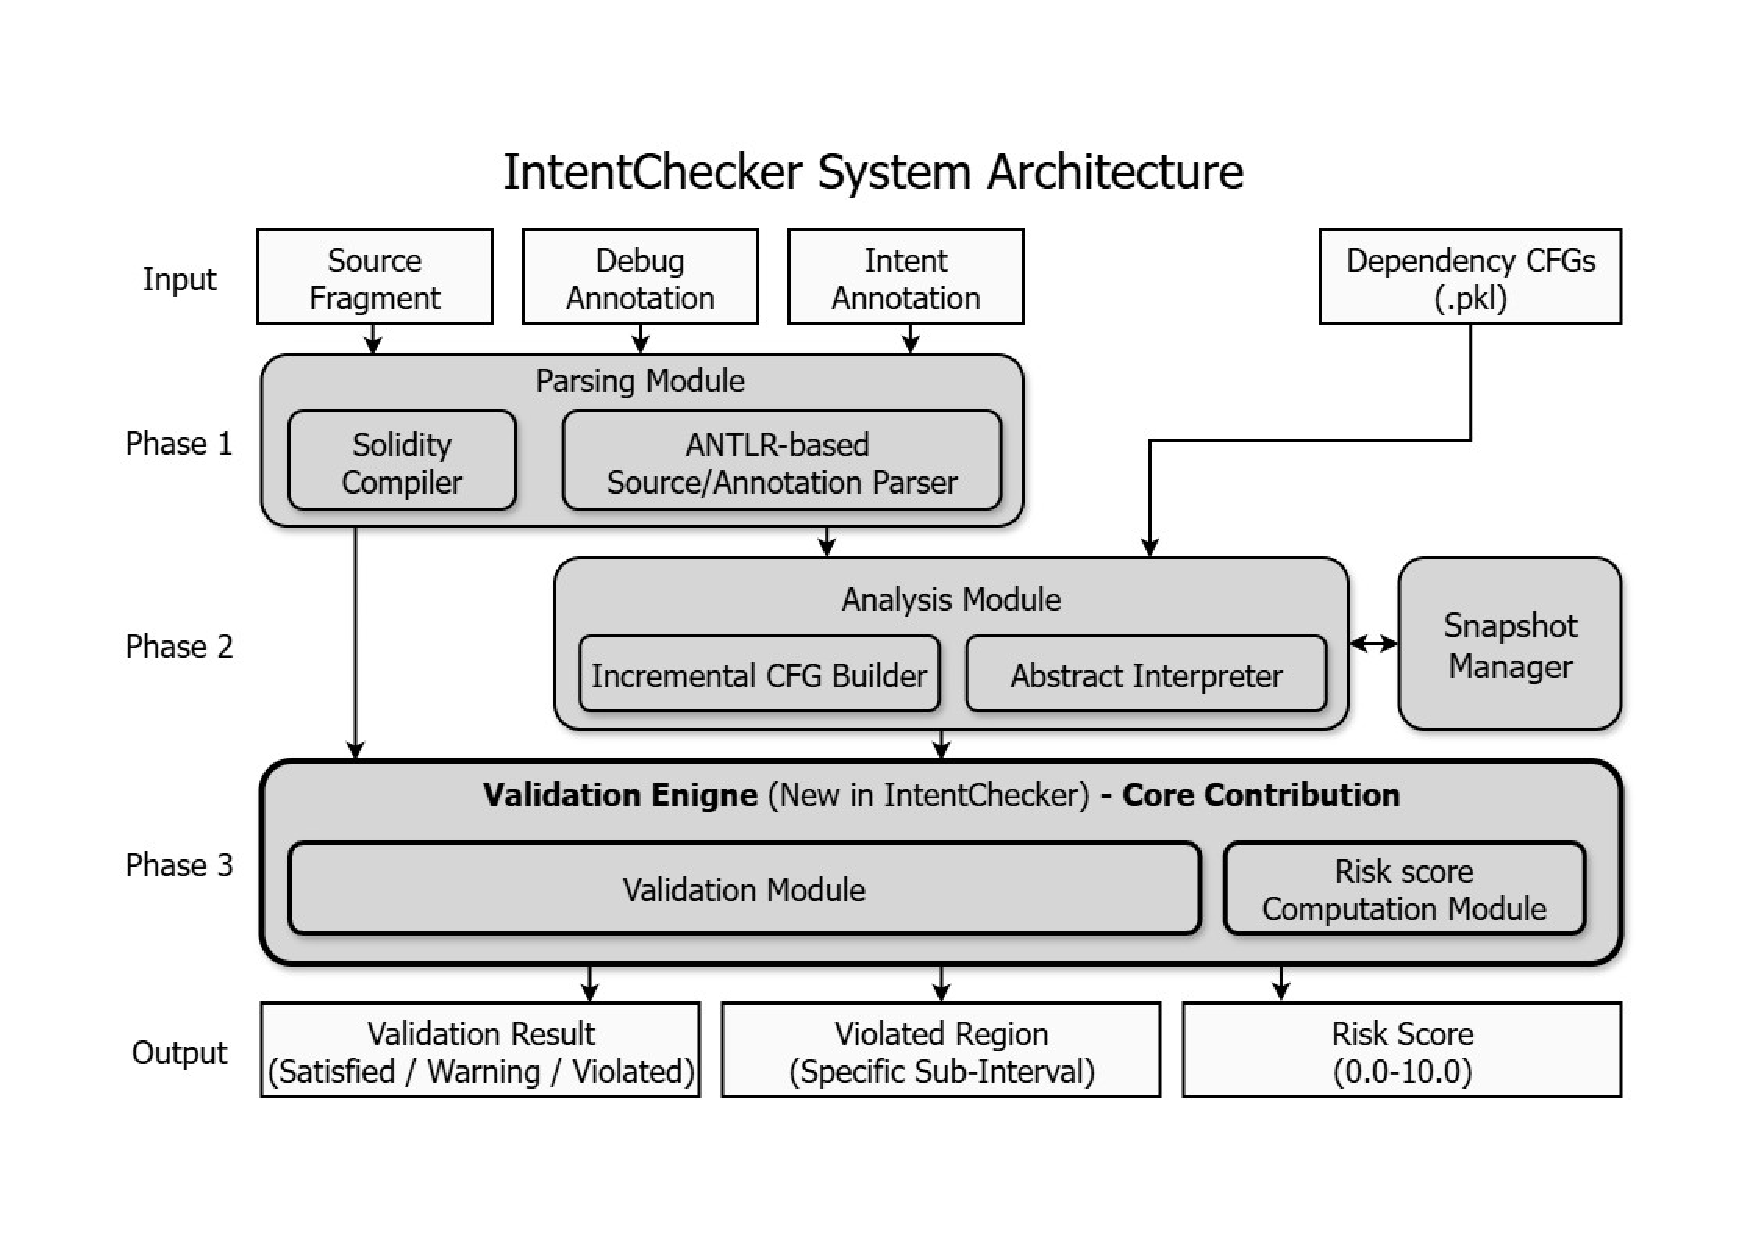
\includegraphics[width=\linewidth]{Fig1.pdf}
    \caption{System architecture of IntentChecker.}
    \label{fig:architecture}
\end{figure}

\smallskip
\noindent\textbf{Internal Modules.}
Phases~1 and~2 reuse and extend SolQDebug's analysis pipeline to accommodate the new @IReturn annotation and the multi-contract deployment-unit scope, while Phase~3 is IntentChecker's core contribution.
\begin{itemize}
    \item \textbf{Phase~1 --- Parsing Module.} Uses ANTLR for syntax analysis of both Solidity source fragments and intent/debug annotation comments, and additionally delegates the Solidity source fragments to the official Solidity compiler for semantic validation.
    \item \textbf{Phase~2 --- Analysis Module.} Performs incremental abstract interpretation over the interval domain, updating the control-flow graph and variable states as each statement is processed. When a debug annotation is received, the Snapshot Manager (reused unchanged from SolQDebug) preserves the current analysis state, allowing the analyzer to overwrite the targeted variable's interval with the developer-supplied range, re-analyze affected code paths, and restore the pre-annotation state afterwards; the same mechanism handles the new @IReturn annotation, since injecting a range at an interface call return site is mechanically the same as injecting one at a @StateVar declaration. The module additionally supports inline assembly written in Yul for arithmetic computation, leaving non-arithmetic constructs at $\top$.
    \item \textbf{Phase~3 --- Validation Engine.} Draws on two signals from the earlier phases---parsed intent annotations from the Parsing Module, which encode the relational constraints declared in @During/@Post annotations, and computed variable intervals from the Analysis Module, which represent the abstract state of each variable at the annotated program point. For each annotation, it evaluates whether the declared intent holds by comparing the actual intervals against the specified constraints, producing the three output fields listed above.
\end{itemize}

\smallskip
\noindent\textbf{Analysis scope.}
IntentChecker analyzes one function at a time within a multi-contract scope, extending SolQDebug's~\citep{solqdebug} original single-contract analysis to cover libraries and inherited parents that share storage with the target contract. External contracts---separately deployed and reached through an address or interface-typed variable---sit outside this scope, because their storage resides at a different address that the target's annotations cannot reach.
This exclusion creates a problem for analysis: any value derived from an interface call resolves to $\top$ and propagates into every downstream computation, defeating intent validation for functions that read oracles or external token state. To address this, @IReturn extends the same range-injection mechanism the three existing annotations rely on: the developer supplies a bounded range for a value the function reads whose origin lies outside the analyzer's view, and the analyzer proceeds under it. Interface functions split into two cases: those declared view or pure, where Solidity guarantees no state-modifying side effects, and those that may modify state---potentially even re-entering the target function. Injection is restricted to the former, allowing intent validation to proceed under the developer-supplied range rather than being defeated by $\top$ propagation.

\subsection{Examples of Intent Annotation Usage}

This section walks through two examples to illustrate how an annotated function produces a validation judgment.
The first case demonstrates a mid-execution check via a @During annotation; the second demonstrates a post-execution check via @Post together with an @IReturn annotation for external contract state.

\smallskip
\noindent\textbf{Case 1: @During --- Operator Order Issue.}
Fig.~\ref{fig:operator-order-example} shows a token purchase function where operator precedence causes the buyer to receive fewer tokens than the exchange rate warrants.

\begin{figure}[t]
\begin{lstlisting}
// contract state: bool presell; uint256 ethRateFix;
// helper: function calculateRate() public view returns (uint256);
function buy() public payable {
    // @GlobalVar msg.value = [50000000000500000, ...]
    // @StateVar presell = true
    require(presell, "presell is closed");
    uint256 amountToBuy = msg.value / ethRateFix * calculateRate();
    // @During amountToBuy * ethRateFix >= msg.value * 250000
    balances[msg.sender] += amountToBuy;
}
\end{lstlisting}
\caption{Operator order issue in exchange rate calculation (simplified).}
\label{fig:operator-order-example}
\end{figure}

The developer's intent is that amountToBuy should satisfy the exchange-rate relation---the tokens received, times the rate denominator, should be at least the ETH paid times the rate numerator.
Because msg.value / ethRateFix truncates before multiplication, this intent is violated for non-round input amounts.
The @During annotation (line~8) captures this intent directly, and IntentChecker reports Violated.

\smallskip
\noindent\textbf{Case 2: @Post --- Erroneous Accounting.}
Fig.~\ref{fig:erroneous-accounting-example} shows a rebasing vault's mint function.
The bug is that minted proxy tokens are computed from the total vault balance (including the just-deposited amount), which inflates the shares beyond the deposited amount when the redeem rate deviates from~1.

\begin{figure}[t]
\begin{lstlisting}
// contract state: uint256 _totalSupply; mapping(address => uint256) _balances;
// address baseToken; uint256 ONE; function redeemRate() public view returns (uint256);
function mint(address to, uint256 amount)
    public override returns (uint256) {
    // @LocalVar amount = [500e18, 500e18]
    // @StateVar _totalSupply = [1000e18, 1000e18]
    // @StateVar _balances[to] = [0, 0]
    // @IReturn IERC20(baseToken).balanceOf()
    //   = [1500e18, 1500e18]
    uint256 _redeemRate = redeemRate();
    require(IERC20(baseToken).transferFrom(
        msg.sender, address(this), amount));
    uint256 baseBalance =
        IERC20(baseToken).balanceOf(address(this));
    uint256 proxy = (baseBalance * ONE) / _redeemRate;
    // @Post _balances[to] <= amount
    _mint(to, proxy);
}
\end{lstlisting}
\caption{Erroneous accounting in vault mint with inflated proxy amount (simplified).}
\label{fig:erroneous-accounting-example}
\end{figure}

The @Post \_balances[to] $\leq$ amount annotation (line~16) expresses the intent that no user should receive more shares than the tokens they deposited.
The @IReturn debug annotation (lines~8--9) injects the range $[1500\,\text{e}18, 1500\,\text{e}18]$ for the external balanceOf call (line~14), which the analyzer would otherwise evaluate as $\top$.
The transferFrom (line~11) is state-modifying and therefore cannot carry an @IReturn annotation, per the view/pure restriction described in §\ref{sec:design}.
With these annotations, IntentChecker computes the proxy amount and finds that it exceeds amount, reporting Violated.
This example demonstrates how @IReturn enables intent validation for functions that depend on external contract state.

\smallskip
These two examples illustrate the two temporal scopes of intent validation---mid-execution checks via @During and post-execution checks via @Post.
The complete intent model supporting these annotations is defined in the following section.

\subsection{Intent Model}\label{sec:intent-model}

The denotational semantics of the intent model is built around a meaning function
\[
\mathcal{V}\llbracket \cdot \rrbracket \;\colon\; \mathbb{A} \;\to\; \bigl(\mathbb{C} \rightharpoonup \mathbb{J}\bigr)
\]
that assigns to each intent annotation $a \in \mathbb{A}$ a partial function from validation contexts to tri-valued judgments. The semantics has three components --- the syntactic domain $\mathbb{A}$, the semantic domain $\mathbb{C}$, and the judgment set $\mathbb{J}$ --- defined as follows.

\smallskip
\noindent\textbf{Syntactic domain.}
$\mathbb{A}$ is the set of intent annotations generated by the grammar of §\ref{sec:intent-semantics}, with a typical element denoted $a$.
Each annotation begins with a marker (@During or @Post) followed by a single body drawn from the corresponding grammatical category.
The grammar partitions bodies into three kinds:
\begin{itemize}
    \item \textbf{@During forms}, attached to an individual statement within the function body, inspect properties at that program point.
    \item \textbf{@Post forms}, evaluated at function exit, inspect function-level properties.
    \item \textbf{Common forms} are shared between the two annotation kinds, applicable in both @During and @Post contexts.
\end{itemize}
There are no compound connectives at the annotation level, so every annotation is atomic.

\smallskip
\noindent\textbf{Semantic domain.}
We use two semantic domains:
\begin{itemize}
    \item $\Sigma$ --- the space of abstract variable environments produced by the interval-domain interpreter. Each $\sigma \in \Sigma$ maps every program variable to an integer interval, or to a compound value (arrays, mappings, or structs) whose leaf components are intervals.
    \item $\mathbb{C}$ --- the set of validation contexts. Each $\Gamma \in \mathbb{C}$ is a record whose fields are listed in Table~\ref{tab:validation-context}; these fields hold the program-state snapshots and auxiliary data the interpreter makes available at an annotated program point, and each annotation form reads only the subset relevant to its form.
\end{itemize}

\begin{table}[t]
\centering
\caption{Fields of the validation context $\Gamma \in \mathbb{C}$. Each atomic annotation form reads only a subset of these fields.}
\label{tab:validation-context}
\small
\begin{tabularx}{\linewidth}{@{} l L @{}}
\toprule
Field & Meaning \\
\midrule
$\sigma_{\text{pt}} \in \Sigma$ & abstract state at the annotated program point \\
$\sigma_{\text{before}} \in \Sigma$ & state immediately before the statement at the annotated line \\
$\sigma_{\text{assign}} \in \Sigma$ & state at a variable's first-assignment site within the enclosing function \\
$\sigma_{\text{entry}} \in \Sigma$ & state at function entry (after parameter binding and debug annotations) \\
$\sigma_{\text{exit}} \in \Sigma$ & joined state at normal function exit \\
$R : \text{Line} \rightharpoonup \text{Val}^*$ & partial map from return-statement lines to captured return values \\
$\mathcal{K}$ & the set of statements at the annotated line (for call-expression and require/assert lookup) \\
$\Pi \subseteq \Sigma$ & the set of abstract states at reachable program points within the enclosing function body, up to the evaluation point \\
\bottomrule
\end{tabularx}
\end{table}

\smallskip
\noindent\textbf{Field supply.}
$\Gamma$ supplies a different subset of fields depending on the annotation kind:
\begin{itemize}
    \item \textbf{@During}: $\sigma_{\text{pt}}$, $\sigma_{\text{before}}$, $\sigma_{\text{assign}}$, $\sigma_{\text{entry}}$, $R$, $\mathcal{K}$, and $\Pi$ (containing every state produced between entry and $\sigma_{\text{pt}}$ along reachable paths);
    \item \textbf{@Post}: $\sigma_{\text{entry}}$, $\sigma_{\text{exit}}$, $R$, and $\Pi$ (containing every state produced along any reachable path from entry to exit).
\end{itemize}

\smallskip
\noindent\textbf{Judgment set.}
$\mathbb{J} = \{S, V, W\}$ is the set of tri-valued judgments assigned to each annotation:
\begin{itemize}
    \item \textbf{Satisfied} ($S$) --- the abstract state guarantees the annotation holds;
    \item \textbf{Violated} ($V$) --- the abstract state guarantees it fails;
    \item \textbf{Warning} ($W$) --- the abstract state admits both satisfying and violating concrete cases.
\end{itemize}
Given an annotation $a \in \mathbb{A}$ whose validation context is $\Gamma \in \mathbb{C}$, IntentChecker reports $\mathcal{V}\llbracket a \rrbracket(\Gamma) \in \mathbb{J}$ as its judgment for that annotation; the partiality of the inner arrow captures the fact that $\mathcal{V}\llbracket a \rrbracket$ is defined only on contexts $\Gamma$ that provide every field $a$ references (see well-formedness in §\ref{sec:intent-semantics}).

The subsection proceeds as follows.
Section~\ref{sec:intent-semantics} fixes the grammar of $\mathbb{A}$ and defines $\mathcal{V}\llbracket \cdot \rrbracket$ via three set-theoretic primitives.
Section~\ref{sec:validation-engine} presents the executable procedures that realise it, with an auxiliary risk score.

\subsubsection{Syntax and Semantics}\label{sec:intent-semantics}

\begin{figure}[t]
\small
\begin{tabular}{@{}r@{\quad}c@{\quad}l@{\qquad}l@{}}
duringIntent & $\rightarrow$ & // @During duringClause & \\[2pt]
postIntent   & $\rightarrow$ & // @Post postClause & \\[6pt]

duringClause & $\rightarrow$ & intentValue (before relOp after)              & $(D_{\text{ba}})$ \\
             & $|$           & intentValue (assign relOp current)            & $(D_{\text{ac}})$ \\
             & $|$           & identifier .arg[ $n$ ] relOp intentValue     & $(D_{\text{arg}})$ \\
             & $|$           & require feasible                              & $(D_{\text{req}})$ \\
             & $|$           & assert feasible                               & $(D_{\text{asrt}})$ \\
             & $|$           & commonClause                                  & $(D_{\text{com}})$ \\[6pt]

postClause & $\rightarrow$ & intentValue (entry relOp exit)                   & $(P_{\text{ee}})$ \\
           & $|$           & commonClause                                     & $(P_{\text{com}})$ \\[6pt]

commonClause & $\rightarrow$ & returnExpression relOp intentValue             & $(C_{\text{ret}})$ \\
             & $|$           & return[$n$] relOp intentValue                  & $(C_{\text{ret}_n})$ \\
             & $|$           & intentValue relOp PercentOf( intentValue , $p$ )  & $(C_{\text{pct}})$ \\
             & $|$           & intentValue relOp ceil( intentValue , $d$ )    & $(C_{\text{ceil}})$ \\
             & $|$           & intentValue relOp floor( intentValue , $d$ )   & $(C_{\text{flr}})$ \\
             & $|$           & intentValue relOp intentValue                   & $(C_{\text{cmp}})$ \\
             & $|$           & intentValue ${=}{>}$ intentValue                & $(C_{\text{impl}})$ \\
             & $|$           & changed ( intentValue , true $|$ false )        & $(C_{\text{chg}})$ \\[6pt]

intentValue & $\rightarrow$ & arithExpr & \\[2pt]
arithExpr   & $\rightarrow$ & arithExpr ($\ll$ $|$ $\gg$ $|$ $\ggg$) arithAdd $|$ arithAdd & \\
arithAdd    & $\rightarrow$ & arithAdd (+ $|$ -) arithTerm $|$ arithTerm & \\
arithTerm   & $\rightarrow$ & arithTerm (* $|$ / $|$ \%) arithExp $|$ arithExp & \\
arithExp    & $\rightarrow$ & arithFactor ** arithExp $|$ arithFactor & \\
arithFactor & $\rightarrow$ & number $|$ [ number , number ] $|$ varRef $|$ ( arithExpr ) & \\[2pt]
varRef      & $\rightarrow$ & identifier subAccess* & \\
subAccess   & $\rightarrow$ & . identifier $|$ [ expr ] & \\[6pt]

relOp & $\rightarrow$ & $<$ $|$ $>$ $|$ $\leq$ $|$ $\geq$ $|$ == $|$ != $|$ in $|$ not in & \\
\end{tabular}
\caption{Grammar of intent annotations. Sub-items of $\mathit{duringClause}$, $\mathit{postClause}$, and $\mathit{commonClause}$ are tagged with rule labels $(D_\bullet)$, $(P_\bullet)$, $(C_\bullet)$ for reference in the text.}
\label{fig:intent-grammar}
\end{figure}

\smallskip
\noindent\textbf{Grammar overview.}
Fig.~\ref{fig:intent-grammar} gives the BNF of intent annotations, embedded in single-line comments so they coexist with Solidity code without affecting compilation.
Intent-value expressions support arithmetic over variable references with member and index access, numeric literals, inline intervals $[a, b]$, and the DSL helpers PercentOf, ceil, and floor.
Relational operators include $<$, $>$, $\leq$, $\geq$, ==, !=, and the membership operators in and not in; the implication operator ${=}{>}$ is a truthiness-based atomic form whose semantics is defined below.

\smallskip
\noindent\textbf{Well-formedness.}
We write $\Gamma \vdash a : \mathbf{wf}$ to mean that annotation $a$ is well-formed under $\Gamma$: $a$ parses against Fig.~\ref{fig:intent-grammar}, every variable reference in $a$ resolves in the relevant field of $\Gamma$, and all form-specific auxiliary data required by $a$ is present in $\Gamma$.
The equations below define $\mathcal{V}\llbracket a \rrbracket(\Gamma)$ only for well-formed inputs; annotation forms whose auxiliary data is missing correspond to error paths in the implementation and lie outside the semantic claim.

Well-formedness is orthogonal to the informativeness of the input intervals themselves.
Debug annotations (@StateVar, @LocalVar, @IReturn), inherited from SolQDebug, are the mechanism by which developers supply bounded ranges for otherwise-unknown variables; without them, interval inputs may remain $\top$, and the primitives defined below typically return $W$ even though the semantics is still sound.

\smallskip
\noindent\textbf{Expression evaluation.}
Let $\mathcal{I}$ denote the set of integer intervals.
Intent-value expressions are evaluated against a chosen abstract variable environment $\sigma \in \Sigma$ by a function
\[
\text{eval} \;:\; \Sigma \times \mathit{intentValue} \;\to\; \mathcal{I},
\]
which delegates to the interpreter's expression evaluator for ordinary arithmetic subexpressions---inheriting soundness of interval arithmetic from the base analyzer---and to annotation-specific rules for the DSL helpers (PercentOf, ceil, floor) and inline interval literals $[a, b]$.
A numeric literal $n$ evaluates to the singleton interval $[n, n]$, so literals never need to live in $\Gamma$.
By contrast, three rules in Fig.~\ref{fig:intent-grammar} whose left-hand sides are not themselves intent-value expressions are handled outside this function: rule $(D_{\text{arg}})$ is reduced by an auxiliary operator $\text{arg}_n(f, \mathcal{K})$ to the actual argument expression---an intent-value expression---which is then passed to $\text{eval}$, while rules $(C_{\text{ret}})$ and $(C_{\text{ret}_n})$ are resolved directly against the return-summary field $R$ as $R(\ell_{\text{ret}})$ and $R(\ell_{\text{ret}})[n]$, respectively, bypassing $\text{eval}$ because $R$ already stores per-line return intervals.

To support the feasibility forms introduced below, we also use the space of abstract boolean intervals $\mathcal{B} = \{\{0\}, \{1\}, \{0, 1\}\}$ and a boolean-expression evaluator
\[
\text{eval}_{\mathcal{B}} \;:\; \Sigma \times \text{BExpr} \;\to\; \mathcal{B},
\]
where $\text{BExpr}$ is not a non-terminal of Fig.~\ref{fig:intent-grammar} but the base language's (Solidity's) boolean-expression category, from which $\text{cond}_{\text{req}}(\mathcal{K})$ and $\text{cond}_{\text{asrt}}(\mathcal{K})$ extract the boolean condition at the annotated line for rules $(D_{\text{req}})$ and $(D_{\text{asrt}})$, respectively; we inherit the soundness of $\text{eval}_{\mathcal{B}}$ from the underlying analyzer.

\smallskip
\noindent\textbf{Comparison primitive.}
Relational annotations are grounded in the set-theoretic comparison primitive
\[
\text{Cmp}^* \;:\; \mathcal{I} \times \text{Op} \times \mathcal{I} \;\to\; \mathbb{J},
\]
defined as
\[
\text{Cmp}^*(L, \mathit{op}, R) \;=\;
\begin{cases}
S & \text{if } \forall l \in L,\ \forall r \in R :\ l \mathrel{\mathit{op}} r, \\[2pt]
V & \text{if } \forall l \in L,\ \forall r \in R :\ \neg(l \mathrel{\mathit{op}} r), \\[2pt]
W & \text{otherwise.}
\end{cases}
\]
For $\mathit{op} \in \{\text{in}, \text{not\,in}\}$, the set-membership interpretation replaces the pointwise comparison: $l \mathrel{\text{in}} R$ holds iff $l \in R$, and not\,in is its complement.
$\text{Cmp}^*$ gives an algorithm-independent specification of what a relational annotation must evaluate to under a well-formed context.

\smallskip
\noindent\textbf{Truthiness implication primitive.}
The implication operator ${=}{>}$ is an atomic form whose two sides are intent-value expressions rather than full annotations; its meaning is grounded in a truthiness-based set-theoretic primitive
\[
\text{Impl}^* \;:\; \mathcal{I} \times \mathcal{I} \;\to\; \mathbb{J},
\]
defined as
\[
\text{Impl}^*(L, R) \;=\;
\begin{cases}
S & \text{if } L = \{0\}, \\[2pt]
S & \text{if } 0 \notin L \text{ and } 0 \notin R, \\[2pt]
V & \text{if } 0 \notin L \text{ and } R = \{0\}, \\[2pt]
W & \text{otherwise.}
\end{cases}
\]
Intuitively, an interval $X$ is definitely non-zero when $0 \notin X$ and definitely zero when $X = \{0\}$.
$\text{Impl}^*(L, R)$ returns $S$ when $L$ is definitely zero (so the implication holds vacuously) or when both sides are definitely non-zero, $V$ when $L$ is definitely non-zero while $R$ is definitely zero, and $W$ when the zero/non-zero status of either side cannot be established.

\smallskip
\noindent\textbf{Feasibility primitive.}
The feasibility forms are grounded in a two-valued primitive over abstract boolean intervals:
\[
\text{Feasible}^* \;:\; \mathcal{B} \;\to\; \mathbb{J}, \qquad
\text{Feasible}^*(B) \;=\;
\begin{cases}
V & \text{if } B = \{0\}, \\
S & \text{otherwise.}
\end{cases}
\]
$\text{Feasible}^*$ answers whether a Solidity boolean condition---as evaluated by $\text{eval}_{\mathcal{B}}$---can ever hold.
When the abstract interval is $\{0\}$, the condition is provably false on every concrete execution, so the underlying statement is unreachable and rules $(D_{\text{req}})$ and $(D_{\text{asrt}})$ yield $V$.
In every other case the condition admits a true value for at least one input, so the statement is feasible and both rules yield $S$.
Unlike $\text{Cmp}^*$ and $\text{Impl}^*$, $\text{Feasible}^*$ is total but two-valued.
Since the question ``is this condition ever true?'' admits no intermediate answer, the warning case of $\mathbb{J}$ is unused.

\smallskip
\noindent\textbf{Meaning function.}
The meaning function $\mathcal{V}\llbracket \cdot \rrbracket$, whose signature was fixed in §\ref{sec:intent-model}, is defined by case analysis over the annotation grammar, one equation per syntactic form.
We use $e$ (possibly subscripted) for an intent-value expression (in the state-comparison and change-detection forms, typically a variable reference, possibly with struct member or mapping index access), $f$ for a function identifier, and $\ell_{\text{ret}}$ for the return-statement line selected by the annotation: in @During, the return statement on the annotated line; in @Post, the join over all return-statement lines recorded in $R$.

\smallskip
\textbf{@During annotations.}
In the equations below, $\text{arg}_n(f, \mathcal{K})$---serving rule $(D_{\text{arg}})$---denotes the $n$-th argument expression of the call to $f$ located within the statements $\mathcal{K}$ at the annotated line (both sides of the comparison are evaluated in $\sigma_{\text{before}}$ because argument values are fixed immediately before the call executes), and $\text{cond}_{\text{req}}(\mathcal{K})$ and $\text{cond}_{\text{asrt}}(\mathcal{K})$---serving rules $(D_{\text{req}})$ and $(D_{\text{asrt}})$---denote the boolean condition expression of the statement located within $\mathcal{K}$ at the annotated line.
\begin{align*}
\mathcal{V}\llbracket e(\text{before}\ \mathit{op}\ \text{after}) \rrbracket(\Gamma)
    &= \text{Cmp}^*\bigl(\text{eval}(\sigma_{\text{before}}, e),\; \mathit{op},\; \text{eval}(\sigma_{\text{pt}}, e)\bigr), \\[3pt]
\mathcal{V}\llbracket e(\text{assign}\ \mathit{op}\ \text{current}) \rrbracket(\Gamma)
    &= \text{Cmp}^*\bigl(\text{eval}(\sigma_{\text{assign}}, e),\; \mathit{op},\; \text{eval}(\sigma_{\text{pt}}, e)\bigr), \\[3pt]
\mathcal{V}\llbracket f.\text{arg}[n]\ \mathit{op}\ e \rrbracket(\Gamma)
    &= \text{Cmp}^*\bigl(\text{eval}(\sigma_{\text{before}}, \text{arg}_n(f, \mathcal{K})),\; \mathit{op},\; \text{eval}(\sigma_{\text{before}}, e)\bigr), \\[3pt]
\mathcal{V}\llbracket \text{require feasible} \rrbracket(\Gamma)
    &= \text{Feasible}^*\bigl(\text{eval}_{\mathcal{B}}(\sigma_{\text{pt}},\; \text{cond}_{\text{req}}(\mathcal{K}))\bigr), \\[3pt]
\mathcal{V}\llbracket \text{assert feasible} \rrbracket(\Gamma)
    &= \text{Feasible}^*\bigl(\text{eval}_{\mathcal{B}}(\sigma_{\text{pt}},\; \text{cond}_{\text{asrt}}(\mathcal{K}))\bigr),
\end{align*}

\smallskip
\textbf{@Post annotations.}
The only @Post-specific rule $(P_{\text{ee}})$ compares the value of $e$ at function entry ($\sigma_{\text{entry}}$) and exit ($\sigma_{\text{exit}}$); the remaining @Post forms are covered by the common-form equations below.
\begin{align*}
\mathcal{V}\llbracket e(\text{entry}\ \mathit{op}\ \text{exit}) \rrbracket(\Gamma)
    &= \text{Cmp}^*\bigl(\text{eval}(\sigma_{\text{entry}}, e),\; \mathit{op},\; \text{eval}(\sigma_{\text{exit}}, e)\bigr).
\end{align*}

\smallskip
\textbf{Common-form annotations.}
For common-form annotations that may appear in either annotation kind, we let $\text{ref}(\Gamma)$ denote the reference environment: $\text{ref}(\Gamma) = \sigma_{\text{pt}}$ under @During and $\text{ref}(\Gamma) = \sigma_{\text{exit}}$ under @Post, capturing the rule that a common-form annotation is evaluated at the annotated program point inside @During but at the function exit inside @Post.
The following equations apply uniformly to annotations of either kind; rules $(C_{\text{pct}})$, $(C_{\text{ceil}})$, and $(C_{\text{flr}})$ are subsumed by rule $(C_{\text{cmp}})$'s general $e_l\ \mathit{op}\ e_r$ equation below, since their right-hand sides are intent-value expressions that $\text{eval}$ handles as DSL-only constructs:
\begin{align*}
\mathcal{V}\llbracket \text{returnExpression}\ \mathit{op}\ e \rrbracket(\Gamma)
    &= \text{Cmp}^*\bigl(R(\ell_{\text{ret}}),\; \mathit{op},\; \text{eval}(\text{ref}(\Gamma), e)\bigr), \\[3pt]
\mathcal{V}\llbracket \text{return}[n]\ \mathit{op}\ e \rrbracket(\Gamma)
    &= \text{Cmp}^*\bigl(R(\ell_{\text{ret}})[n],\; \mathit{op},\; \text{eval}(\text{ref}(\Gamma), e)\bigr), \\[3pt]
\mathcal{V}\llbracket e_l\ \mathit{op}\ e_r \rrbracket(\Gamma)
    &= \text{Cmp}^*\bigl(\text{eval}(\text{ref}(\Gamma), e_l),\; \mathit{op},\; \text{eval}(\text{ref}(\Gamma), e_r)\bigr), \\[3pt]
\mathcal{V}\llbracket e_l \Rightarrow e_r \rrbracket(\Gamma)
    &= \text{Impl}^*\bigl(\text{eval}(\text{ref}(\Gamma), e_l),\; \text{eval}(\text{ref}(\Gamma), e_r)\bigr).
\end{align*}

The change-detection form $\text{changed}(e, b)$ of rule $(C_{\text{chg}})$ asks whether $e$ has been modified at any reachable program point within the function body relative to its entry value.
Its meaning is therefore not a single $\text{Cmp}^*$ call between two states but a quantification over $\Pi$, lifting $\text{Cmp}^*$ with operator $=$ to the ``exists-a-witness'' reading:
\begin{align*}
\mathcal{V}\llbracket \text{changed}(e, \text{true}) \rrbracket(\Gamma) \;=\;
\begin{cases}
S & \text{if } \exists \sigma \in \Pi : \text{Cmp}^*\bigl(\text{eval}(\sigma_{\text{entry}}, e),\; =,\; \text{eval}(\sigma, e)\bigr) = V, \\[2pt]
V & \text{if } \forall \sigma \in \Pi : \text{Cmp}^*\bigl(\text{eval}(\sigma_{\text{entry}}, e),\; =,\; \text{eval}(\sigma, e)\bigr) = S, \\[2pt]
W & \text{otherwise.}
\end{cases}
\end{align*}
The dual form, asking that $e$ be unchanged throughout the function body, is defined by swapping $S$ and $V$:
\begin{align*}
\mathcal{V}\llbracket \text{changed}(e, \text{false}) \rrbracket(\Gamma) \;=\;
\begin{cases}
S & \text{if } \forall \sigma \in \Pi : \text{Cmp}^*\bigl(\text{eval}(\sigma_{\text{entry}}, e),\; =,\; \text{eval}(\sigma, e)\bigr) = S, \\[2pt]
V & \text{if } \exists \sigma \in \Pi : \text{Cmp}^*\bigl(\text{eval}(\sigma_{\text{entry}}, e),\; =,\; \text{eval}(\sigma, e)\bigr) = V, \\[2pt]
W & \text{otherwise.}
\end{cases}
\end{align*}
Because $\Pi$ is populated differently for @During (states from entry up to the annotated point) and @Post (states from entry up to any exit), these two equations cover both annotation kinds with a single pair of cases; no separate equations per kind are needed.

\subsubsection{Auxiliary Outputs: Violated Region and Risk Score}\label{sec:validation-engine}

\begin{algorithm}[!t]
\caption{Auxiliary Outputs Computation for $\text{Cmp}^*$-based Annotations}
\label{alg:risk-score}
\begin{algorithmic}[1]
\State \textbf{Input:} Intervals $L$, $R$, operator $op$, state $j \in \mathbb{J}$
\State \textbf{Output:} $(\mathit{risk\_score},\; \mathit{regions})$ with $\mathit{risk\_score} \in [0.0, 10.0]$ and $\mathit{regions} = (L_{\mathit{lower}}, L_{\mathit{upper}}, L_{\mathit{overlap}})$
\State $(|T_s|, |T_v|, |T_w|) \gets \mathit{RegionSizes}(L, R, op)$
\State $\mathit{regions} \gets \mathit{ExtractViolatedRegion}(L, R, op)$
\If{$j = \mathit{satisfied}$}
    \State \Return $(0.0,\; \mathit{regions})$
\ElsIf{$j = \mathit{violated}$}
    \State \Return $(10.0,\; \mathit{regions})$
\EndIf
\State $p \gets p_{\mathit{true}}(L, R, op)$
\State $\mathit{risk\_type} \gets \mathit{ClassifyRisk}(\mathit{regions},\, op)$
\State $(\mathit{base},\, \mathit{span}) \gets \mathit{BandOf}(\mathit{risk\_type})$
\State $\mathit{risk\_score} \gets \mathit{base} + (1 - p) \times \mathit{span}$
\State \Return $(\mathit{risk\_score},\; \mathit{regions})$
\end{algorithmic}
\end{algorithm}

This subsection presents the executable procedures that accompany the semantic realisation of §\ref{sec:intent-semantics}, producing two auxiliary outputs derived from the same interval analysis that drives $\text{Cmp}^*$:
\begin{itemize}
    \item \textbf{violated region} --- sub-intervals of the input range $L$ that witness the failure of the comparison;
    \item \textbf{risk score} --- a value on a 0--10 scale combining the state, the true probability, and the shape of the violated region.
\end{itemize}

Both outputs are downstream of the semantic claim and do not refine the judgment $j \in \mathbb{J}$; they support warning ranking and developer feedback.
An internal probability $p_{\mathit{true}}(L, R, op) \in [0, 1]$ --- the chance that the comparison holds under a uniform distribution over $L \times R$ --- mediates the risk-score computation but is not surfaced separately.
$\text{Impl}^*$ and $\text{Feasible}^*$ are directly computable from their definitions and need no dedicated algorithm, and the change-detection form iterates $\Pi$ directly.
The remaining auxiliary outputs for $\text{Cmp}^*$-based annotations are computed by Algorithm~\ref{alg:risk-score} in four steps, each elaborated in turn below and cited with its line range in the algorithm.

\smallskip
\noindent\textbf{Step 1: Region partitioning (Algorithm~\ref{alg:risk-score}, line 3).}
Given integer intervals $L = [l_{\min}, l_{\max}]$ and $R = [r_{\min}, r_{\max}]$ with an operator $op$, the interpreter partitions $L$ into three disjoint regions:
\begin{itemize}
    \item $T_s$ (satisfied region): values of $L$ for which $l \mathrel{op} r$ holds for all $r \in R$;
    \item $T_v$ (violated region): values of $L$ for which $l \mathrel{op} r$ fails for all $r \in R$;
    \item $T_w$ (warning region): values of $L$ whose truth value depends on the actual value of $R$.
\end{itemize}

Table~\ref{tab:op-formulas} gives the satisfied/violated conditions and region sizes per operator, where $n_L = l_{\max} - l_{\min} + 1$ and $n_R = r_{\max} - r_{\min} + 1$ denote the number of integer values in each interval.
The state $j$ returned by $\text{Cmp}^*$ follows directly: $j = S$ when the satisfied condition holds, $j = V$ when the violated condition holds, and $j = W$ when neither holds.
Fig.~\ref{fig:region-partition} illustrates this partition for $op = \text{``$>$''}$ across the spectrum of $L$ vs $R$ relative positions on the integer line: from $L$ entirely below $R$ (Verdict: Violated) through several warning configurations to $L$ entirely above $R$ (Verdict: Satisfied). The same Table~\ref{tab:op-formulas} formulas apply throughout, with $\max(0, \cdot)$ clamping handling the empty regions in each configuration.

\begin{table}[t]
\centering
\caption{Per-operator satisfied/violated conditions and region sizes. All sizes are clamped to $\max(0, \cdot)$.}
\label{tab:op-formulas}
\small
\begin{tabular}{cllcc}
\toprule
$op$ & Satisfied condition & Violated condition & $|T_s|$ & $|T_v|$ \\
\midrule
$>$    & $l_{\min} > r_{\max}$    & $l_{\max} \leq r_{\min}$  & $l_{\max} - r_{\max}$     & $r_{\min} - l_{\min} + 1$ \\
$\geq$ & $l_{\min} \geq r_{\max}$ & $l_{\max} < r_{\min}$     & $l_{\max} - r_{\max} + 1$ & $r_{\min} - l_{\min}$     \\
$<$    & $l_{\max} < r_{\min}$    & $l_{\min} \geq r_{\max}$  & $r_{\min} - l_{\min}$     & $l_{\max} - r_{\max} + 1$ \\
$\leq$ & $l_{\max} \leq r_{\min}$ & $l_{\min} > r_{\max}$     & $r_{\min} - l_{\min} + 1$ & $l_{\max} - r_{\max}$     \\
\midrule
$=$    & $L = R$, both singletons  & $L \cap R = \emptyset$  & $|L \cap R|$ & $n_L - |L \cap R|$ \\
$\neq$ & $L \cap R = \emptyset$  & $L = R$, both singletons  & $n_L - |L \cap R|$ & $|L \cap R|$ \\
\midrule
in     & $L \subseteq R$ & $L \cap R = \emptyset$ & $|L \cap R|$       & $n_L - |L \cap R|$ \\
not\,in & $L \cap R = \emptyset$ & $L \subseteq R$ & $n_L - |L \cap R|$ & $|L \cap R|$       \\
\bottomrule
\end{tabular}
\end{table}

\begin{figure}[t]
\centering

% Row 1: (a) L below R, (b) L extends below R
\begin{subfigure}[b]{0.48\linewidth}
\centering
\begin{tikzpicture}[
    x=0.3cm, y=0.4cm,
    Rbox/.style={fill=red!30, draw=red!60!black, line width=0.4pt},
    Tsbox/.style={fill=green!40, draw=green!60!black, line width=0.4pt},
    Tvbox/.style={fill=red!50, draw=red!65!black, line width=0.4pt},
    Twbox/.style={fill=yellow!60, draw=orange!65!black, line width=0.4pt},
    ax/.style={->, line width=0.4pt, black!70},
    tick/.style={line width=0.3pt, black!70},
    txt/.style={font=\tiny},
    Tlbl/.style={font=\scriptsize},
]
\fill[Rbox] (8, 5.0) rectangle (12, 6.0);
\node[Tlbl] at (10, 5.5) {$R$};
\draw[tick] (8, 4.8) -- (8, 6.2);
\draw[tick] (12, 4.8) -- (12, 6.2);
\node[txt, anchor=south] at (8, 6.2) {$r_{\min}$};
\node[txt, anchor=south] at (12, 6.2) {$r_{\max}$};
\fill[Tvbox] (2, 3.0) rectangle (6, 4.0);
\node[Tlbl] at (4, 3.5) {$T_v$};
\node[Tlbl, anchor=east] at (1.8, 3.5) {$L$};
\draw[tick] (2, 2.8) -- (2, 4.2);
\draw[tick] (6, 2.8) -- (6, 4.2);
\node[txt, anchor=north] at (2, 2.8) {$l_{\min}$};
\node[txt, anchor=north] at (6, 2.8) {$l_{\max}$};
\draw[ax] (0, 2.0) -- (20, 2.0);
\node[txt, anchor=west] at (20, 2.0) {$\mathbb{Z}$};
\end{tikzpicture}
\caption{$L$ below $R$: $T_v = L$ (Violated).}
\label{fig:region-fullyv}
\end{subfigure}
\hfill
\begin{subfigure}[b]{0.48\linewidth}
\centering
\begin{tikzpicture}[
    x=0.3cm, y=0.4cm,
    Rbox/.style={fill=red!30, draw=red!60!black, line width=0.4pt},
    Tsbox/.style={fill=green!40, draw=green!60!black, line width=0.4pt},
    Tvbox/.style={fill=red!50, draw=red!65!black, line width=0.4pt},
    Twbox/.style={fill=yellow!60, draw=orange!65!black, line width=0.4pt},
    ax/.style={->, line width=0.4pt, black!70},
    tick/.style={line width=0.3pt, black!70},
    txt/.style={font=\tiny},
    Tlbl/.style={font=\scriptsize},
]
\fill[Rbox] (8, 5.0) rectangle (12, 6.0);
\node[Tlbl] at (10, 5.5) {$R$};
\draw[tick] (8, 4.8) -- (8, 6.2);
\draw[tick] (12, 4.8) -- (12, 6.2);
\node[txt, anchor=south] at (8, 6.2) {$r_{\min}$};
\node[txt, anchor=south] at (12, 6.2) {$r_{\max}$};
\fill[Tvbox] (4, 3.0) rectangle (8, 4.0);
\fill[Twbox] (8, 3.0) rectangle (10, 4.0);
\node[Tlbl] at (6, 3.5) {$T_v$};
\node[Tlbl] at (9, 3.5) {$T_w$};
\node[Tlbl, anchor=east] at (3.8, 3.5) {$L$};
\draw[tick] (4, 2.8) -- (4, 4.2);
\draw[tick] (10, 2.8) -- (10, 4.2);
\node[txt, anchor=north] at (4, 2.8) {$l_{\min}$};
\node[txt, anchor=north] at (10, 2.8) {$l_{\max}$};
\draw[ax] (0, 2.0) -- (20, 2.0);
\node[txt, anchor=west] at (20, 2.0) {$\mathbb{Z}$};
\end{tikzpicture}
\caption{$L$ extends below $R$: $T_s = \emptyset$ (Warning).}
\label{fig:region-lower}
\end{subfigure}

\vspace{8pt}

% Row 2: (c) L inside R, (d) L surrounds R (canonical)
\begin{subfigure}[b]{0.48\linewidth}
\centering
\begin{tikzpicture}[
    x=0.3cm, y=0.4cm,
    Rbox/.style={fill=red!30, draw=red!60!black, line width=0.4pt},
    Tsbox/.style={fill=green!40, draw=green!60!black, line width=0.4pt},
    Tvbox/.style={fill=red!50, draw=red!65!black, line width=0.4pt},
    Twbox/.style={fill=yellow!60, draw=orange!65!black, line width=0.4pt},
    ax/.style={->, line width=0.4pt, black!70},
    tick/.style={line width=0.3pt, black!70},
    txt/.style={font=\tiny},
    Tlbl/.style={font=\scriptsize},
]
\fill[Rbox] (8, 5.0) rectangle (12, 6.0);
\node[Tlbl] at (10, 5.5) {$R$};
\draw[tick] (8, 4.8) -- (8, 6.2);
\draw[tick] (12, 4.8) -- (12, 6.2);
\node[txt, anchor=south] at (8, 6.2) {$r_{\min}$};
\node[txt, anchor=south] at (12, 6.2) {$r_{\max}$};
\fill[Twbox] (9, 3.0) rectangle (11, 4.0);
\node[Tlbl] at (10, 3.5) {$T_w$};
\node[Tlbl, anchor=east] at (8.8, 3.5) {$L$};
\draw[tick] (9, 2.8) -- (9, 4.2);
\draw[tick] (11, 2.8) -- (11, 4.2);
\node[txt, anchor=north] at (9, 2.8) {$l_{\min}$};
\node[txt, anchor=north] at (11, 2.8) {$l_{\max}$};
\draw[ax] (0, 2.0) -- (20, 2.0);
\node[txt, anchor=west] at (20, 2.0) {$\mathbb{Z}$};
\end{tikzpicture}
\caption{$L$ inside $R$: $T_w = L$ (Warning).}
\label{fig:region-Rcontains}
\end{subfigure}
\hfill
\begin{subfigure}[b]{0.48\linewidth}
\centering
\begin{tikzpicture}[
    x=0.3cm, y=0.4cm,
    Rbox/.style={fill=red!30, draw=red!60!black, line width=0.4pt},
    Tsbox/.style={fill=green!40, draw=green!60!black, line width=0.4pt},
    Tvbox/.style={fill=red!50, draw=red!65!black, line width=0.4pt},
    Twbox/.style={fill=yellow!60, draw=orange!65!black, line width=0.4pt},
    ax/.style={->, line width=0.4pt, black!70},
    tick/.style={line width=0.3pt, black!70},
    txt/.style={font=\tiny},
    Tlbl/.style={font=\scriptsize},
]
\fill[Rbox] (8, 5.0) rectangle (12, 6.0);
\node[Tlbl] at (10, 5.5) {$R$};
\draw[tick] (8, 4.8) -- (8, 6.2);
\draw[tick] (12, 4.8) -- (12, 6.2);
\node[txt, anchor=south] at (8, 6.2) {$r_{\min}$};
\node[txt, anchor=south] at (12, 6.2) {$r_{\max}$};
\fill[Tvbox] (4, 3.0) rectangle (8, 4.0);
\fill[Twbox] (8, 3.0) rectangle (12, 4.0);
\fill[Tsbox] (12, 3.0) rectangle (16, 4.0);
\node[Tlbl] at (6, 3.5) {$T_v$};
\node[Tlbl] at (10, 3.5) {$T_w$};
\node[Tlbl] at (14, 3.5) {$T_s$};
\node[Tlbl, anchor=east] at (3.8, 3.5) {$L$};
\draw[tick] (4, 2.8) -- (4, 4.2);
\draw[tick] (16, 2.8) -- (16, 4.2);
\node[txt, anchor=north] at (4, 2.8) {$l_{\min}$};
\node[txt, anchor=north] at (16, 2.8) {$l_{\max}$};
\draw[ax] (0, 2.0) -- (20, 2.0);
\node[txt, anchor=west] at (20, 2.0) {$\mathbb{Z}$};
\end{tikzpicture}
\caption{$L$ surrounds $R$ (canonical): all three regions non-empty (Warning).}
\label{fig:region-canonical}
\end{subfigure}

\vspace{8pt}

% Row 3: (e) L extends above R, (f) L above R
\begin{subfigure}[b]{0.48\linewidth}
\centering
\begin{tikzpicture}[
    x=0.3cm, y=0.4cm,
    Rbox/.style={fill=red!30, draw=red!60!black, line width=0.4pt},
    Tsbox/.style={fill=green!40, draw=green!60!black, line width=0.4pt},
    Tvbox/.style={fill=red!50, draw=red!65!black, line width=0.4pt},
    Twbox/.style={fill=yellow!60, draw=orange!65!black, line width=0.4pt},
    ax/.style={->, line width=0.4pt, black!70},
    tick/.style={line width=0.3pt, black!70},
    txt/.style={font=\tiny},
    Tlbl/.style={font=\scriptsize},
]
\fill[Rbox] (8, 5.0) rectangle (12, 6.0);
\node[Tlbl] at (10, 5.5) {$R$};
\draw[tick] (8, 4.8) -- (8, 6.2);
\draw[tick] (12, 4.8) -- (12, 6.2);
\node[txt, anchor=south] at (8, 6.2) {$r_{\min}$};
\node[txt, anchor=south] at (12, 6.2) {$r_{\max}$};
\fill[Twbox] (10, 3.0) rectangle (12, 4.0);
\fill[Tsbox] (12, 3.0) rectangle (16, 4.0);
\node[Tlbl] at (11, 3.5) {$T_w$};
\node[Tlbl] at (14, 3.5) {$T_s$};
\node[Tlbl, anchor=east] at (9.8, 3.5) {$L$};
\draw[tick] (10, 2.8) -- (10, 4.2);
\draw[tick] (16, 2.8) -- (16, 4.2);
\node[txt, anchor=north] at (10, 2.8) {$l_{\min}$};
\node[txt, anchor=north] at (16, 2.8) {$l_{\max}$};
\draw[ax] (0, 2.0) -- (20, 2.0);
\node[txt, anchor=west] at (20, 2.0) {$\mathbb{Z}$};
\end{tikzpicture}
\caption{$L$ extends above $R$: $T_v = \emptyset$ (Warning).}
\label{fig:region-upper}
\end{subfigure}
\hfill
\begin{subfigure}[b]{0.48\linewidth}
\centering
\begin{tikzpicture}[
    x=0.3cm, y=0.4cm,
    Rbox/.style={fill=red!30, draw=red!60!black, line width=0.4pt},
    Tsbox/.style={fill=green!40, draw=green!60!black, line width=0.4pt},
    Tvbox/.style={fill=red!50, draw=red!65!black, line width=0.4pt},
    Twbox/.style={fill=yellow!60, draw=orange!65!black, line width=0.4pt},
    ax/.style={->, line width=0.4pt, black!70},
    tick/.style={line width=0.3pt, black!70},
    txt/.style={font=\tiny},
    Tlbl/.style={font=\scriptsize},
]
\fill[Rbox] (8, 5.0) rectangle (12, 6.0);
\node[Tlbl] at (10, 5.5) {$R$};
\draw[tick] (8, 4.8) -- (8, 6.2);
\draw[tick] (12, 4.8) -- (12, 6.2);
\node[txt, anchor=south] at (8, 6.2) {$r_{\min}$};
\node[txt, anchor=south] at (12, 6.2) {$r_{\max}$};
\fill[Tsbox] (14, 3.0) rectangle (18, 4.0);
\node[Tlbl] at (16, 3.5) {$T_s$};
\node[Tlbl, anchor=east] at (13.8, 3.5) {$L$};
\draw[tick] (14, 2.8) -- (14, 4.2);
\draw[tick] (18, 2.8) -- (18, 4.2);
\node[txt, anchor=north] at (14, 2.8) {$l_{\min}$};
\node[txt, anchor=north] at (18, 2.8) {$l_{\max}$};
\draw[ax] (0, 2.0) -- (20, 2.0);
\node[txt, anchor=west] at (20, 2.0) {$\mathbb{Z}$};
\end{tikzpicture}
\caption{$L$ above $R$: $T_s = L$ (Satisfied).}
\label{fig:region-fullys}
\end{subfigure}

\caption{Spectrum of $L$ vs $R$ configurations for $op = \text{``$>$''}$.}
\label{fig:region-partition}
\end{figure}

\smallskip
\noindent\textbf{Step 2: Violated-region extraction (Algorithm~\ref{alg:risk-score}, line 4).}
The interpreter also extracts the violated region of $L$: sub-intervals of $L$ that witness failure.
Table~\ref{tab:false-regions} decomposes $L$ into three directional components per operator:
\begin{itemize}
    \item $L_{\mathit{lower}}$ --- values of $L$ that fall below the acceptable range of $R$;
    \item $L_{\mathit{upper}}$ --- values of $L$ that exceed the acceptable range of $R$;
    \item $L_{\mathit{overlap}}$ --- values of $L$ whose outcome depends on the concrete $R$-value (the warning region for ordering operators; the coincidence zone for equality/membership).
\end{itemize}

Each component is an integer sub-interval or empty; empty components indicate that no witness exists in that direction.
For the $=$ operator, when $L$ and $R$ are disjoint, the overlap is empty and $L$ falls entirely into exactly one of $L_{\mathit{lower}}$ or $L_{\mathit{upper}}$ depending on which side it lies on.
The risk-classification step below consumes this decomposition, and the same sub-intervals are surfaced to the developer as the concrete ranges where the annotation may fail.

\begin{table}[t]
\centering
\caption{Violated-region extraction formulas. Endpoints are clamped so that $\min > \max$ yields empty; ``---'' denotes no witness in that direction.}
\label{tab:false-regions}
\footnotesize
\begin{tabular*}{\linewidth}{@{\extracolsep{\fill}} c l l l @{}}
\toprule
$op$ & $L_{\mathit{lower}}$ & $L_{\mathit{upper}}$ & $L_{\mathit{overlap}}$ \\
\midrule
$>$    & $[l_{\min}, \min(l_{\max}, r_{\min})]$         & ---                                             & $[\max(l_{\min}, r_{\min}{+}1), \min(l_{\max}, r_{\max})]$ \\
$\geq$ & $[l_{\min}, \min(l_{\max}, r_{\min}{-}1)]$     & ---                                             & $[\max(l_{\min}, r_{\min}), \min(l_{\max}, r_{\max})]$ \\
$<$    & ---                                            & $[\max(l_{\min}, r_{\max}), l_{\max}]$          & $[\max(l_{\min}, r_{\min}), \min(l_{\max}, r_{\max}{-}1)]$ \\
$\leq$ & ---                                            & $[\max(l_{\min}, r_{\max}{+}1), l_{\max}]$      & $[\max(l_{\min}, r_{\min}), \min(l_{\max}, r_{\max})]$ \\
\midrule
$=$    & $[l_{\min}, (L \cap R)_{\min}{-}1]$            & $[(L \cap R)_{\max}{+}1, l_{\max}]$             & $L \cap R$ \\
$\neq$ & ---                                            & ---                                             & $L \cap R$ \\
\midrule
\text{in}      & $[l_{\min}, \min(l_{\max}, r_{\min}{-}1)]$ & $[\max(l_{\min}, r_{\max}{+}1), l_{\max}]$  & --- \\
\text{not\,in} & ---                                    & ---                                             & $L \cap R$ \\
\bottomrule
\end{tabular*}
\end{table}

\smallskip
\noindent\textbf{Step 3: State-based scoring (Algorithm~\ref{alg:risk-score}, lines 5--9).}
Lines 5--9 map the state $j$ returned by $\text{Cmp}^*$ directly to extreme scores: $j = \mathit{satisfied}$ returns $0.0$ (fully satisfied condition) and $j = \mathit{violated}$ returns $10.0$ (definite violation).
The warning case $j = W$ requires further composition and is handled in Step~4.

\smallskip
\noindent\textbf{Step 4: Warning-case scoring (Algorithm~\ref{alg:risk-score}, lines 10--13).}
When $j = W$, the risk score is composed from an internal probability $p_{\mathit{true}}$ and a risk-type classification over the violated-region components, then assembled into a value in $(0.0, 10.0)$ by a banded linear formula.

\smallskip
\textbf{True probability (Algorithm~\ref{alg:risk-score}, line 10).}
The true probability $p_{\mathit{true}}(L, R, op) \in [0, 1]$ that the comparison holds under a uniform distribution over $L \times R$ is defined in closed form using the region sizes from Step~1:
\[
p_{\mathit{true}}(L, R, op) \;=\;
\begin{cases}
|T_s| / n_L & \text{if } op \in \{\text{in}, \text{not\,in}\}, \\[3pt]
|T_s| / (n_L \cdot n_R) & \text{if } op = \text{``=''} \text{ and } n_R > 1, \\[3pt]
1 - |T_v| / (n_L \cdot n_R) & \text{if } op = \text{``$\neq$''} \text{ and } n_R > 1, \\[3pt]
\bigl(|T_s| + E_w\bigr) / n_L & \text{otherwise.}
\end{cases}
\]

\begin{figure}[t]
\centering

% Row 1: (a) L extends below R, (b) L inside R
\begin{subfigure}[b]{0.48\linewidth}
\centering
\begin{tikzpicture}[
    x=0.4cm, y=0.3cm,
    bar/.style={fill=orange!55, draw=orange!75!black, line width=0.4pt},
    ax/.style={->, line width=0.4pt, black!70},
    pair/.style={dashed, blue!60!black, line width=0.5pt},
    rRef/.style={dotted, black!50, line width=0.4pt},
    txt/.style={font=\tiny},
]
\draw[rRef] (0, -0.3) -- (0, 8);
\draw[rRef] (6, -0.3) -- (6, 8);
\node[txt, anchor=north] at (0, -0.3) {$r_{\min}$};
\node[txt, anchor=north] at (6, -0.3) {$r_{\max}$};
\foreach \x/\h in {1/1, 2/2, 3/3, 4/4} {
  \fill[bar] (\x-0.3, 0) rectangle (\x+0.3, \h);
}
\draw[pair, <->] (1, 1.2) to[bend left=30] (4, 4.2);
\draw[pair, <->] (2, 2.2) to[bend left=20] (3, 3.2);
\node[txt, blue!60!black] at (2.5, 5.8) {$a+b=5$};
\draw[ax] (-0.5, 0) -- (7.5, 0);
\node[txt, anchor=west] at (7.5, 0) {$l$};
\node[txt, anchor=east] at (0.6, 1) {$a$};
\node[txt, anchor=east] at (0.6, 4) {$b$};
\end{tikzpicture}
\caption{$L$ extends below $R$: $|T_w|=4$, $a{=}1$, $b{=}4$.}
\label{fig:arith-lower}
\end{subfigure}
\hfill
\begin{subfigure}[b]{0.48\linewidth}
\centering
\begin{tikzpicture}[
    x=0.4cm, y=0.3cm,
    bar/.style={fill=orange!55, draw=orange!75!black, line width=0.4pt},
    ax/.style={->, line width=0.4pt, black!70},
    pair/.style={dashed, blue!60!black, line width=0.5pt},
    rRef/.style={dotted, black!50, line width=0.4pt},
    txt/.style={font=\tiny},
]
\draw[rRef] (0, -0.3) -- (0, 8);
\draw[rRef] (6, -0.3) -- (6, 8);
\node[txt, anchor=north] at (0, -0.3) {$r_{\min}$};
\node[txt, anchor=north] at (6, -0.3) {$r_{\max}$};
\foreach \x/\h in {2/2, 3/3, 4/4, 5/5} {
  \fill[bar] (\x-0.3, 0) rectangle (\x+0.3, \h);
}
\draw[pair, <->] (2, 2.2) to[bend left=30] (5, 5.2);
\draw[pair, <->] (3, 3.2) to[bend left=20] (4, 4.2);
\node[txt, blue!60!black] at (3.5, 6.8) {$a+b=7$};
\draw[ax] (-0.5, 0) -- (7.5, 0);
\node[txt, anchor=west] at (7.5, 0) {$l$};
\node[txt, anchor=east] at (1.6, 2) {$a$};
\node[txt, anchor=east] at (1.6, 5) {$b$};
\end{tikzpicture}
\caption{$L$ inside $R$: $|T_w|=4$, $a{=}2$, $b{=}5$.}
\label{fig:arith-inside}
\end{subfigure}

\vspace{8pt}

% Row 2: (c) L surrounds R (canonical), (d) L extends above R
\begin{subfigure}[b]{0.48\linewidth}
\centering
\begin{tikzpicture}[
    x=0.4cm, y=0.3cm,
    bar/.style={fill=orange!55, draw=orange!75!black, line width=0.4pt},
    ax/.style={->, line width=0.4pt, black!70},
    pair/.style={dashed, blue!60!black, line width=0.5pt},
    rRef/.style={dotted, black!50, line width=0.4pt},
    txt/.style={font=\tiny},
]
\draw[rRef] (0, -0.3) -- (0, 8);
\draw[rRef] (6, -0.3) -- (6, 8);
\node[txt, anchor=north] at (0, -0.3) {$r_{\min}$};
\node[txt, anchor=north] at (6, -0.3) {$r_{\max}$};
\foreach \x/\h in {1/1, 2/2, 3/3, 4/4, 5/5, 6/6} {
  \fill[bar] (\x-0.3, 0) rectangle (\x+0.3, \h);
}
\draw[pair, <->] (1, 1.2) to[bend left=35] (6, 6.2);
\draw[pair, <->] (2, 2.2) to[bend left=25] (5, 5.2);
\draw[pair, <->] (3, 3.2) to[bend left=15] (4, 4.2);
\node[txt, blue!60!black] at (3.5, 8.5) {$a+b=7$};
\draw[ax] (-0.5, 0) -- (7.5, 0);
\node[txt, anchor=west] at (7.5, 0) {$l$};
\node[txt, anchor=east] at (0.6, 1) {$a$};
\node[txt, anchor=east] at (0.6, 6) {$b$};
\end{tikzpicture}
\caption{$L$ surrounds $R$ (canonical): $|T_w|=6$, $a{=}1$, $b{=}6$.}
\label{fig:arith-canonical}
\end{subfigure}
\hfill
\begin{subfigure}[b]{0.48\linewidth}
\centering
\begin{tikzpicture}[
    x=0.4cm, y=0.3cm,
    bar/.style={fill=orange!55, draw=orange!75!black, line width=0.4pt},
    ax/.style={->, line width=0.4pt, black!70},
    pair/.style={dashed, blue!60!black, line width=0.5pt},
    rRef/.style={dotted, black!50, line width=0.4pt},
    txt/.style={font=\tiny},
]
\draw[rRef] (0, -0.3) -- (0, 8);
\draw[rRef] (6, -0.3) -- (6, 8);
\node[txt, anchor=north] at (0, -0.3) {$r_{\min}$};
\node[txt, anchor=north] at (6, -0.3) {$r_{\max}$};
\foreach \x/\h in {3/3, 4/4, 5/5, 6/6} {
  \fill[bar] (\x-0.3, 0) rectangle (\x+0.3, \h);
}
\draw[pair, <->] (3, 3.2) to[bend left=30] (6, 6.2);
\draw[pair, <->] (4, 4.2) to[bend left=20] (5, 5.2);
\node[txt, blue!60!black] at (4.5, 8) {$a+b=9$};
\draw[ax] (-0.5, 0) -- (7.5, 0);
\node[txt, anchor=west] at (7.5, 0) {$l$};
\node[txt, anchor=east] at (2.6, 3) {$a$};
\node[txt, anchor=east] at (2.6, 6) {$b$};
\end{tikzpicture}
\caption{$L$ extends above $R$: $|T_w|=4$, $a{=}3$, $b{=}6$.}
\label{fig:arith-upper}
\end{subfigure}

\caption{Arithmetic-sequence visualization of $E_w$ across warning configurations for $op = \text{``$>$''}$ with $n_R = 7$.}
\label{fig:arithmetic-series}
\end{figure}

\begin{itemize}
\item For $op \in \{\text{in}, \text{not\,in}\}$, $|T_s|$ already counts the $L$-values inside $R$, yielding $|T_s|/n_L$ directly.
\item For $op = \text{``=''}$ or $\text{``$\neq$''}$ with $n_R > 1$, each overlapping $L$-value has a $1/n_R$ probability of matching any particular $R$-value, so satisfying pairs are counted over the product space and divided by $n_L \cdot n_R$ (all pairs).
\item Otherwise (when $op \in \{>, \geq, <, \leq\}$, or $=$/$\neq$ with $n_R = 1$), the warning region $T_w$ is the range of $L$-values whose outcome depends on $R$.
Since Solidity operates on integers, for each $l \in T_w$ the number of $R$-values satisfying $l \mathrel{op} r$ forms an arithmetic sequence across $T_w$. Fig.~\ref{fig:arithmetic-series} visualizes this sequence across the four warning configurations identified in Fig.~\ref{fig:region-partition}; in each panel, pairing symmetric terms (first with last, second with second-to-last, and so on) yields a constant pair-sum equal to $a + b$, so the $|T_w|$ counts sum to $(a+b)|T_w|/2$, and dividing by $n_R$ gives
\[
E_w \;=\; \frac{(a + b) \, |T_w|}{2 \, n_R},
\]
where $a$ and $b$ are the numbers of satisfying $R$-values at the smallest and largest elements of $T_w$, respectively.
When $n_R = 1$ for $=$ or $\neq$, $E_w = 0$ and the formula degenerates to pointwise evaluation.
\end{itemize}

\smallskip
\textbf{Risk type classification (Algorithm~\ref{alg:risk-score}, line 11).}
For warning results, the engine classifies the violation pattern into three risk types based on which components of Table~\ref{tab:false-regions} are non-empty:
\begin{itemize}
    \item \textbf{Type 1} --- no directional witness in $L_{\mathit{lower}}$ or $L_{\mathit{upper}}$ (only an overlap zone, representing a mild uncertainty);
    \item \textbf{Type 2} --- exactly one of $L_{\mathit{lower}}$ or $L_{\mathit{upper}}$ is non-empty (a single-direction violation);
    \item \textbf{Type 3} --- both $L_{\mathit{lower}}$ and $L_{\mathit{upper}}$ are non-empty, or the operator is $=$/$\neq$ (whose interval semantics is inherently imprecise and is assigned the highest band by convention).
\end{itemize}

\smallskip
\textbf{Banded scoring (Algorithm~\ref{alg:risk-score}, lines 12--13).}
Each type maps to a fixed $(\mathit{base}, \mathit{span})$ band --- $(0.1, 3.2)$ for type~1, $(3.4, 3.2)$ for type~2, $(6.7, 3.2)$ for type~3 --- and the final score within the band is $\mathit{base} + (1 - p_{\mathit{true}}) \times \mathit{span}$, so that a lower $p_{\mathit{true}}$ (a more probable violation) yields a higher score.

\smallskip
This banded structure is designed for at-a-glance interpretability: $0$ marks safe execution, $10$ a certain violation, and the three bands group warnings by structural severity---mild overlap-only ambiguity (Type~1), single-direction violation (Type~2), and full bilateral or imprecise comparison (Type~3). Developers can therefore prioritize reviews directly by score without inspecting the underlying probability or region structure.

This completes the design of IntentChecker's intent model and validation engine. The full implementation, together with the evaluation benchmark and scripts used in the following section, is publicly available~\citep{intentchecker}.

\section{Evaluation}\label{sec:evaluation}

IntentChecker is evaluated through three research questions that probe its empirical mitigation capability, the structural reasons behind unmitigated cases, and its position relative to existing detection tools:

\begin{itemize}
    \item \textbf{RQ1 (Mitigation Capability)}: Can intent-model-based validation provide developers with actionable diagnostic signals for numeric logic errors during development?
    \item \textbf{RQ2 (Unmitigated Case Analysis)}: For instances that the tool cannot handle, what is the structural reason, and how does this distribute across limitation types?
    \item \textbf{RQ3 (Comparison with Existing Detection Tools)}: How does IntentChecker's approach compare to existing detection tools in terms of detection model, coverage, and analysis latency?
\end{itemize}

\subsection{Experimental Setup}\label{sec:setup}

\noindent\textbf{Experimental Setting.}
The evaluation environment consists of an 11th Gen Intel\textregistered{} Core\texttrademark{}
i7-11390H CPU at 3.40\,GHz with 16.0\,GB RAM, running Windows 10 (64-bit).

\smallskip
\noindent\textbf{Implementation and Execution.}
IntentChecker is implemented in Python~3.10, and operates directly on Solidity source code without requiring compilation or deployment.
Although IntentChecker is designed for interactive use inside a Solidity editor, all experiments simulate this behavior in a controlled scripting environment: for each function, a sequence of incremental edits and annotations reproducing realistic developer activity is reconstructed and streamed into the interpreter, so that the per-case latency reported in \S\ref{sec:rq3} reflects the same per-annotation analysis budget the tool targets in-editor.

\smallskip
\noindent\textbf{Dataset Collection.}
A benchmark of 89 real-world numeric logic error instances is constructed from three complementary sources, each contributing different error patterns under IntentChecker's scope (multi-contract / single-transaction).

\smallskip\noindent\textbf{NumScout (7 instances).}
NumScout~\citep{numscout} provides a curated collection of numeric logic errors mined from deployed BNB Smart Chain contracts.
From the 95-sample subset distributed in NumScout's official repository~\citep{numscout_dataset}---which the authors identify as their main case-level evaluation set---seven cases are selected covering all five numerical defect patterns enumerated in NumScout (Div In Path, Operator Order Issue, Exchange Problem, Precision Loss Trend, and Minor Amount Retention), with two instances for Precision Loss Trend and two for Exchange Problem---one of which is labeled Profit Opportunity in the repository.
All selected contracts target Solidity~$\geq$0.6, the minimum version supported by IntentChecker's front-end; one contract carries a 0.4.x pragma but uses only constructs semantically identical under $\geq$0.6.

\smallskip\noindent\textbf{Flyinointment (1 instance).}
One Greedy Contract instance from the dataset of \citet{flyinointment} is additionally included; that dataset originally introduced the Greedy Contract pattern and is referenced in §\ref{sec:background}.1.

\smallskip\noindent\textbf{Web3Bugs (81 instances).}
Web3Bugs~\citep{exploitablebugs} systematically collected and classified high-severity vulnerabilities from Code4rena audit contests.
Bugs whose execution context fits IntentChecker's scope---multi-contract single-transaction numeric logic errors---are drawn from (i) categories S6-1 through S6-4 (Erroneous Accounting), whose root causes are semantic errors in arithmetic or accounting logic, and (ii) category S3-1 (Inconsistent State Updates), retaining only the subset whose root cause involves a numeric computation with a missing or stale state variable update.
The resulting Web3Bugs subset contains 81 instances spanning Erroneous Accounting (72) and Inconsistent State Updates (9).

\begin{table}[t]
\centering
\caption{Benchmark dataset composition.}
\label{tab:dataset}
\begin{tabular*}{\linewidth}{@{\extracolsep{\fill}} l l r @{}}
\toprule
\textbf{Source} & \textbf{Error Pattern} & \textbf{Count} \\
\midrule
\multirow{5}{*}{NumScout}
  & Div In Path              & 1  \\
  & Exchange Problem         & 2  \\
  & Operator Order Issue     & 1  \\
  & Precision Loss Trend     & 2  \\
  & Minor Amount Retention   & 1  \\
\midrule
Flyinointment & Greedy Contract & 1 \\
\midrule
\multirow{2}{*}{Web3Bugs}
  & Erroneous Accounting        & 72 \\
  & Inconsistent State Updates  & 9  \\
\midrule
\textbf{Total (collected)} & & \textbf{89} \\
Excluded (see below)        & & $-14$ \\
\textbf{Effective}          & & \textbf{75} \\
\bottomrule
\end{tabular*}
\end{table}

\smallskip\noindent\textbf{Exclusions.}
Of the 89 collected instances, 14 are excluded after manual inspection because they fall outside the definition of a development-time numeric logic error.
The exclusion categories are:
\begin{itemize}
  \item \textbf{E1 (Source already patched, 2).} The provided source code is a post-fix version; the reported bug cannot be reproduced.
  \item \textbf{E2 (Integer overflow/underflow, 2).} The program reverts via Solidity~$\geq$0.8 checked arithmetic rather than returning a wrong value, so no numeric logic error is observable at the output level.
  \item \textbf{E3 (Duplicate, 2).} Duplicate audit findings on the same buggy site.
  \item \textbf{E4 (Not a bug, 1).} The project sponsor disputed the finding as intended behavior.
  \item \textbf{E5 (Missing dependency, 2).} Required external libraries not provided in the audit package.
  \item \textbf{E6 (Multi-transaction, 3).} Outside the scope of this study: the bug requires state changes across separate transactions, which IntentChecker's single-transaction analysis cannot cover.
  \item \textbf{E7 (Language semantics, 1).} The reported issue is an inherent property of Solidity's integer-only arithmetic (truncating division), not a developer error; no alternative implementation can produce a different result.
  \item \textbf{Bug not in target contract (1).} The bug actually resides in a different contract than the one documented in the audit report.
\end{itemize}
The remaining \textbf{75 instances} form the effective evaluation set used in RQ1--RQ3.

\subsection{RQ1: Mitigation Capability}\label{sec:rq1}

\begin{table}[t]
\centering
\caption{Evaluation outcome for the 75 effective benchmark instances. Top: the 20 mitigated cases by annotation form. Bottom: the 55 not\_detectable cases by limitation type (sub-categories defined in §\ref{sec:rq2}).}
\label{tab:rq1-overview}
\small
\begin{tabular*}{\linewidth}{@{\extracolsep{\fill}} l l r @{}}
\toprule
\textbf{Outcome} & \textbf{Detail} & \textbf{Cases} \\
\midrule
\multicolumn{3}{@{}l}{\textbf{Mitigated (20)}} \\
\addlinespace
\multicolumn{3}{@{}l}{\quad @During (12)} \\
& Relational comparison (var relOp expr)        & 5 \\
& Before/After (var(Before relOp After))        & 2 \\
& Function-arg check (func.arg[N] relOp expr)  & 3 \\
& Implication form                              & 1 \\
& Feasibility check (require feasible)          & 1 \\
\addlinespace
\multicolumn{3}{@{}l}{\quad @Post (8)} \\
& Relational comparison (var relOp expr)        & 4 \\
& Entry/Exit (var(Entry relOp Exit))            & 2 \\
& Return expression (returnExpression relOp expr) & 1 \\
& changed(var, true/false)                      & 1 \\
\midrule
\multicolumn{3}{@{}l}{\textbf{Not detectable (55)}} \\
\addlinespace
& L1: Loop-related precision loss               & 10 \\
& L2: Interface / external call returns $\top$  & 4 \\
& L3: Unsupported construct                     & 7 \\
& L4: Inexpressible intent                      & 20 \\
& L5: Bug-awareness required                    & 14 \\
\midrule
\multicolumn{2}{@{}l}{\textbf{Total}} & \textbf{75} \\
\bottomrule
\end{tabular*}
\end{table}

\begin{table}[t]
\centering
\caption{Per-case analysis time on the 20 mitigated cases (mean over 3 runs, single thread, dependency pre-analysis excluded). Cases sorted by mean time.}
\label{tab:rq1-timing}
\small
\begin{tabular}{l l r r}
\toprule
\textbf{Case} & \textbf{Error Pattern} & \textbf{Mean (s)} & \textbf{Range (s)} \\
\midrule
div\_in\_path\_WANGMI             & Div In Path              & 14.94 & 12.0--16.8 \\
web3bugs\_45\_H\_01               & Erroneous Acct.          & 13.55 & 9.4--18.4  \\
web3bugs\_58\_H\_02               & Erroneous Acct.          &  9.67 & 7.0--13.8  \\
indivisible\_amount\_BoostToken   & Minor Amt.\ Retention    &  5.67 & 5.0--6.1   \\
operator\_order\_issue\_BoostToken& Operator Order Issue      &  5.43 & 4.9--5.8   \\
web3bugs\_62\_H\_08               & Inconsist.\ State Upd.   &  4.76 & 4.4--5.1   \\
web3bugs\_70\_H\_10               & Inconsist.\ State Upd.   &  3.32 & 3.0--3.6   \\
web3bugs\_51\_H\_02               & Erroneous Acct.          &  3.18 & 2.8--4.0   \\
web3bugs\_56\_H\_02               & Erroneous Acct.          &  2.37 & 1.5--4.0   \\
profit\_opportunity\_HIT          & Exchange Problem         &  2.03 & 1.6--2.5   \\
web3bugs\_5\_H\_12                & Erroneous Acct.          &  1.75 & 0.9--3.4   \\
web3bugs\_47\_H\_02               & Erroneous Acct.          &  1.42 & 1.3--1.5   \\
web3bugs\_5\_H\_08                & Erroneous Acct.          &  1.10 & 1.0--1.3   \\
web3bugs\_60\_H\_01               & Erroneous Acct.          &  1.06 & 1.0--1.1   \\
web3bugs\_101\_H\_01              & Erroneous Acct.          &  0.87 & 0.8--0.9   \\
exchange\_problem\_Nokon          & Exchange Problem         &  0.67 & 0.6--0.8   \\
greedy\_contract\_SwordCrowdsale  & Greedy Contract          &  0.66 & 0.6--0.7   \\
web3bugs\_78\_H\_02               & Erroneous Acct.          &  0.58 & 0.6--0.6   \\
web3bugs\_5\_H\_07                & Erroneous Acct.          &  0.44 & 0.3--0.6   \\
web3bugs\_77\_H\_01               & Erroneous Acct.          &  0.33 & 0.3--0.4   \\
\midrule
\textbf{Mean of means} & & \textbf{3.69} & --- \\
\bottomrule
\end{tabular}
\end{table}

\begin{figure}[t]
\centering
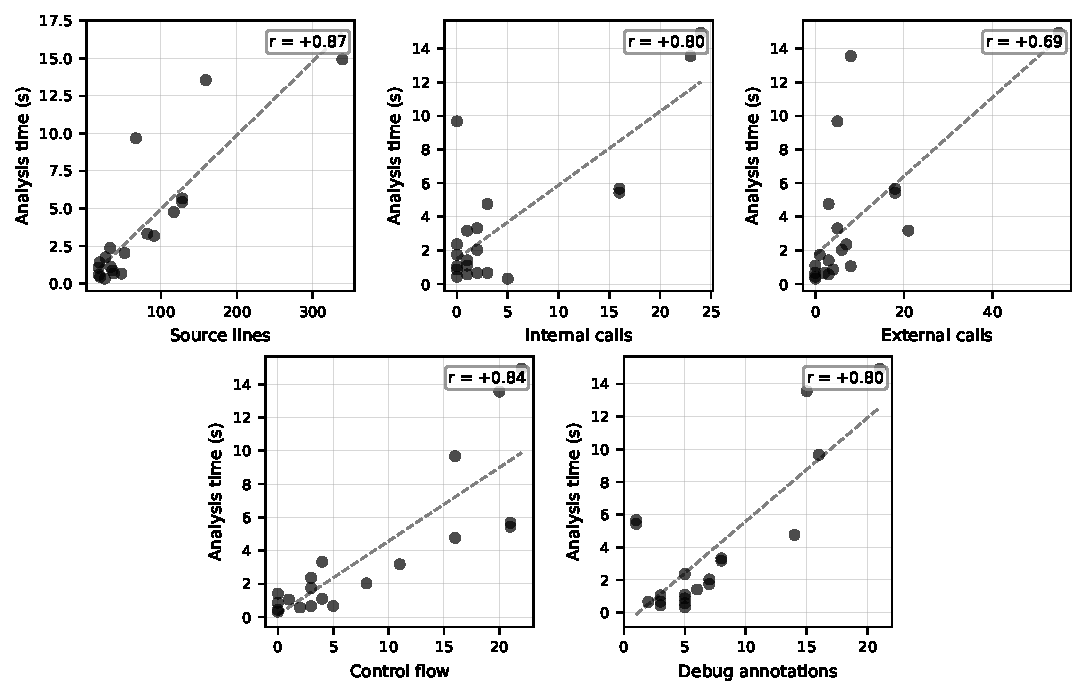
\includegraphics[width=\linewidth]{Fig7.pdf}
\caption{Scatter plots of per-case analysis time against six complexity metrics (20 mitigated cases, 3-run mean). Dashed lines show linear regression; $r$ is the Pearson correlation coefficient.}
\label{fig:rq1-scatter}
\end{figure}

\noindent\textbf{Setup.}
For each of the 75 effective benchmark instances (§\ref{sec:setup}), the evaluation procedure comprised four steps: (1) reading the accompanying bug documentation and identifying the buggy line(s), (2) writing @During and/or @Post intent annotations that capture the expected numeric behavior described therein, (3) supplying the debug annotations (@StateVar, @LocalVar, @GlobalVar, and @IReturn) that the function needs to be analyzable under representative inputs, and (4) running IntentChecker on the resulting annotated source.
The judgment produced by the validation engine---Satisfied, Warning, or Violated---was recorded together with the risk score and violated region.
For instances where no annotation drives the validation engine to Violated on the buggy code, the structural reason was further classified according to the limitation taxonomy in RQ2 (§\ref{sec:rq2}).

\smallskip
\noindent\textbf{Outcomes.}
Of the 75 effective instances, IntentChecker produces a Violated judgment on \textbf{20 cases} when supplied with annotations derived from the bug documentation.
The remaining 55 instances are classified as not\_detectable: no annotation can drive the validation engine to Violated on the buggy code, given the structure of its analysis or its intent model.
Table~\ref{tab:rq1-overview} summarizes the full outcome distribution; the structural reasons behind the 55 unmitigated cases are analyzed in RQ2 (§\ref{sec:rq2}).

\smallskip
\noindent\textbf{Annotation model usage on the 20 mitigated cases.}
The upper half of Table~\ref{tab:rq1-overview} reports which intent annotations were used to surface the bug in each mitigated case.
Of the 20 cases, 12 use a @During annotation (mid-execution checks) and 8 use a @Post annotation (post-execution checks).
The single most common form is the simple relational comparison (intentValue relOp intentValue), used in 9 cases across both @During and @Post.
The two specialized @During forms---Before/After comparisons against an injection point, and func.arg[N] checks on argument values---are each used 2--3 times, and the specialized @Post forms (Entry/Exit, returnExpression, changed(\,)) account for the remainder.
This distribution suggests that the bulk of mitigation work in our benchmark is carried by the basic relational form, with the specialized annotations contributing on patterns that the basic form cannot capture (e.g., monotonicity over function execution, argument-level constraints, post-execution change detection).

\smallskip
\noindent\textbf{Pattern coverage of the 20 mitigated cases.}
As shown in the Error Pattern column of Table~\ref{tab:rq1-timing}, the 20 mitigated instances cover 7 of the 8 single-transaction error patterns enumerated in §\ref{sec:background}.1: Div In Path, Operator Order Issue, Exchange Problem, Minor Amount Retention, Erroneous Accounting (with both Wrong Interest Rate Order and Wrong Checkpoint Order sub-patterns appearing), Inconsistent State Updates, and Greedy Contract.
Precision Loss Trend is present in the benchmark (2 cases) but both instances are not mitigated.
The coverage across 7 of 8 patterns indicates that mitigability depends on whether the error is expressible as an intent violation, not on the error's classification---suggesting that intent-based validation is pattern-agnostic in scope.

\smallskip
\noindent\textbf{Analysis time and what drives it.}
Per-case end-to-end analysis time was measured over three independent runs of each mitigated case on a single thread, excluding the one-time dependency pre-analysis phase (inherited contracts and libraries are pre-analyzed and their control-flow graphs are stored as serialized objects, so they need not be rebuilt across editing sessions).
The mean per-case time is \textbf{3.69\,s}, the minimum is 0.33\,s (web3bugs\_77\_H\_01), and the maximum is 14.94\,s (div\_in\_path\_WANGMI); 15 of the 20 cases finish in under 5\,s, and all but two finish in under 10\,s.
The full per-case timings appear in Table~\ref{tab:rq1-timing}.

To understand what drives the variation across cases, five per-case complexity metrics were collected and the Pearson correlation coefficient $r$~\citep{pearson_r} of each was computed against the 3-run mean analysis time $\bar{y}_i$.
For two variables $X$ (metric) and $Y$ (analysis time) with $n$ paired observations $\{(x_i,y_i)\}_{i=1}^{n}$,
\[
  r \;=\; \frac{\sum_{i}(x_i-\bar{x})(y_i-\bar{y})}
               {\sqrt{\sum_{i}(x_i-\bar{x})^{2}}\;\cdot\;\sqrt{\sum_{i}(y_i-\bar{y})^{2}}}\,,
  \qquad -1 \le r \le +1\,,
\]
where $r=+1$ indicates a perfect positive linear relationship and $r=0$ indicates no linear association.

Fig.~\ref{fig:rq1-scatter} plots each metric against analysis time.
Four of the five metrics exhibit a strong positive correlation ($r>0.8$):
\begin{itemize}
  \item \textbf{Source lines} ($r=0.87$) is the strongest predictor, as it directly reflects the amount of code the abstract interpreter must traverse.
  \item \textbf{Control flow} ($r=0.84$), the aggregate count of loops, branches, and guards (require/assert), increases the number of join operations and fixpoint iterations the abstract interpreter must perform.
  \item \textbf{Internal calls} ($r=0.80$) captures the depth of the call chain within the contraction. Each internal call requires the abstract interpreter to enter a new function scope, propagate abstract states across the call boundary, and merge the return state back into the caller.
  \item \textbf{Debug annotations} ($r=0.80$) adds tracked variables to the abstract state, increasing per-step cost proportionally.
\end{itemize}
The consistently strong correlation across these four metrics ($r \ge 0.80$, $n=20$) suggests that analysis time scales approximately linearly with the size and complexity of the analysis input within the range observed in our benchmark.
Within this trend, the three slowest cases combine the metrics differently: div\_in\_path\_WANGMI and web3bugs\_45\_H\_01 are at the upper end of source-line count and internal-call depth, while web3bugs\_58\_H\_02 owes its 9.7\,s time to four loops---more than any other case---whose fixpoint iterations dominate the abstract interpreter's per-case cost despite a shorter body.
The remaining metric, by contrast, departs from this linear pattern:
\begin{itemize}
  \item \textbf{External calls} ($r=0.69$) shows a comparatively weaker correlation. Dependencies are excluded from per-case time as noted above, and interface function calls lack an implementation body, so the analyzer resolves them to $\top$ or a user-supplied @IReturn value without traversal.
\end{itemize}

Taken together, RQ1 shows that intent-based validation can surface actionable diagnostic signals for 20 of 75 benchmark instances across 7 of 8 error patterns, with per-case analysis completing in under 15\,s (mean 3.69\,s) and scaling proportionally with code complexity.
These results suggest that IntentChecker is practical as a development-time validation tool for numeric logic errors in smart contracts.

\subsection{RQ2: Unmitigated Case Analysis}\label{sec:rq2}

\noindent\textbf{Overview.}
RQ2 classifies the 55 instances for which IntentChecker cannot produce a Violated judgment on the buggy code into analysis-engine limitations (L1--L3) and annotation-grammar limitations (L4--L5), and further examines the expressibility of the annotation grammar within L4--L5 (Fig.~\ref{fig:rq1-limitations}).

\begin{figure}[t]
\centering
\begin{tikzpicture}[font=\small]
  % Constants
  \def\barH{0.45}
  \def\barGap{0.30}  % widened for vertical readability
  \def\xUnit{0.30}   % cm per case (accommodates max=20)
  \def\maxCount{20}

  % Group A: analysis-engine (L1-L3)
  \def\colA{black!55}
  % Group B: annotation-level (L4, L5)
  \def\colB{black!25}

  % Bars: (index/label/count/color/type name)
  \foreach \i/\lab/\val/\col/\desc in {%
    0/L1a/8/\colA/Loop widening,
    1/L1b/2/\colA/Loop body granularity,
    2/L2a/3/\colA/Interface call return $\top$,
    3/L2b/1/\colA/External call unknown state,
    4/L3/7/\colA/Unsupported construct,
    5/L4/20/\colB/Grammar expressibility limit,
    6/L5/14/\colB/Bug-awareness limit%
  } {%
    \pgfmathsetmacro{\y}{-\i*(\barH+\barGap)}
    \pgfmathsetmacro{\w}{\val*\xUnit}
    \node[anchor=east] at (0,\y) {\textbf{\lab}};
    \fill[\col] (0.15,\y-\barH/2) rectangle (0.15+\w,\y+\barH/2);
    \node[anchor=west] at (0.18+\w,\y) {\val\;\scriptsize\desc};
  }

  % Group brackets (bars 0-4 = L1a-L3, bars 5-6 = L4-L5)
  \draw[thick] (-1.05,0.32) -- (-1.15,0.32) -- (-1.15,-3.28) -- (-1.05,-3.28);
  \node[rotate=90, anchor=south, align=center] at (-1.25,-1.48) {\scriptsize Analysis\\engine (21)};
  \draw[thick] (-1.05,-3.47) -- (-1.15,-3.47) -- (-1.15,-4.82) -- (-1.05,-4.82);
  \node[rotate=90, anchor=south, align=center] at (-1.25,-4.145) {\scriptsize Annotation\\level (34)};

  % X-axis
  \draw[->] (0.15,-5.45) -- (0.15+21*\xUnit,-5.45);
  \foreach \x in {0,5,10,15,20} {
    \draw (0.15+\x*\xUnit,-5.40) -- (0.15+\x*\xUnit,-5.50);
    \node[anchor=north] at (0.15+\x*\xUnit,-5.50) {\scriptsize \x};
  }
  \node[anchor=north] at (0.15+10*\xUnit,-5.85) {\scriptsize \# of cases};
\end{tikzpicture}
\caption{Limitation breakdown for the 55 not\_detectable instances: analysis-engine limits (L1--L3, 21) vs.\ annotation-level limits (L4, L5, 34).}
\label{fig:rq1-limitations}
\end{figure}

\smallskip
\noindent\textbf{Limitation type definitions.}
\begin{itemize}
  \item \textbf{L1--L3 (Analysis-engine limits, 21 cases).}
  \begin{itemize}
    \item \textbf{L1a (Loop widening, 8).} A variable that the bug check depends on is widened to $\top$ inside a preceding loop, and the $\top$ propagates past the loop exit to the check point.
    \item \textbf{L1b (Loop body granularity, 2).} The bug manifests at a specific point inside a loop body, but the analyzer's state at that point is a single summary joined over all iterations. Per-iteration observation is not a check point the intent annotation model exposes.
    \item \textbf{L2a (Interface call return $\top$, 3).} The bug check depends on a value derived from a state-modifying interface call. The implementation is unavailable and @IReturn applies only to view/pure calls (§\ref{sec:design}), so the return collapses to $\top$ and propagates to the check point.
    \item \textbf{L2b (External call, unknown external state, 1).} The bug check depends on the return of a cross-contract call whose implementation is available through dependency pre-analysis. An L1, L2a, or L3 pattern within the callee's own body causes $\top$ to propagate to its return value, which then reaches the check point.
    \item \textbf{L3 (Unsupported construct, 7).} The bug check depends on a value that flows through an unsupported construct---abi.decode, opaque hash builtins, or non-arithmetic Yul---which the analyzer treats as $\top$, and the $\top$ propagates to the check point.
  \end{itemize}
  \noindent In these 21 cases, the analyzer's state at the check point is too coarse to distinguish the bug---either a $\top$ value (L1a, L2a, L2b, L3) or a summary joined across loop iterations (L1b). Such a state spans both the developer's intended range and outside it, so the annotation evaluates to Warning rather than Violated---an ambiguous judgment that applies equally to the buggy and bug-free code. They are residual failures after the analyzer's precision mechanisms---annotation-guided adaptive widening inherited from SolQDebug~\citep{solqdebug}, debug-annotation-supplied symbolic values, and dependency pre-analysis for cross-contract resolution---have been applied. The presence of a loop, an external call, or a low-level construct does not by itself block analysis. L1--L3 arise only when the bug-relevant state at the check point falls into one of the specific failure modes enumerated above.

  \item \textbf{L4--L5 (Annotation-layer limits, 34 cases).}
  \begin{itemize}
    \item \textbf{L4 (Grammar expressibility limit, 20 cases).} The annotation grammar targets relationships among the variables the target function uses. The correct specification for these cases lies outside that scope---typically because it requires referencing external computations or variables the function does not use.
    \item \textbf{L5 (Bug-awareness limit, 14 cases).} The correct specification lies within the annotation grammar's scope---it can be written as a relationship among the variables the target function uses. Writing it requires the developer to articulate the intended relationship with enough precision to distinguish it from the buggy one, which in practice presupposes having already recognized the bug.
  \end{itemize}

  \noindent To distinguish the bug patterns IntentChecker's value-level intent model can address from those that fall outside its scope, the 34 cases are classified along two orthogonal axes. The first is the Value/Algorithm distinction introduced in §\ref{sec:background}.1 (Table~\ref{tab:nle-patterns}): whether the bug lies at the value level (a wrong operator, swapped identifier, or missing assignment) or at the algorithm level (operation ordering, missing procedure call). The second is the reference location, classifying each case by whether the corrective reference is reachable from the target function:
  \begin{itemize}
    \item \textbf{Usable.} The reference is bound to a variable the function already reads, such as a local variable, parameter, or contract state variable.
    \item \textbf{Unusable.} The reference is bound elsewhere, such as in external contract state, in the return of a call the function does not make, or in no variable the program represents at all.
  \end{itemize}

  \noindent The four resulting cells partition the 34 cases. Each cell is illustrated below with a representative bug from our benchmark.
  \begin{itemize}
    \item \textbf{Value / Usable (13).} An in-function variable holds the correct value or relation, but the buggy code references the wrong one, or a state update that should have named a specific variable is missing. Twelve cases are L5, and one is an L4 case where the grammar cannot express the exact magnitude of the required state transition. In 113\_H\_05 (NFTPairWithOracle.\_lend), the buggy require statement reverses the intended comparison between offer.ltvBPS and userProfile.maxLTV, and both are in-scope parameters of the function.
    \item \textbf{Value / Unusable (8).} No in-function variable stands in for the correct value needed at the check point. All eight cases are L4. In 25\_H\_05 (CTokenMultiOracle.\_setSource), the function hardcodes 18 as the price-feed decimals. The correct value would come from calling the feed's decimals function, which the target function never does.
    \item \textbf{Algorithm / Usable (3).} All relevant variables are in scope, but the correct specification is a structural relation---a multi-variable invariant, an operation ordering, or a missing helper call---that the grammar does not directly support. Two cases are L5, and one is an L4 case requiring arithmetic over Entry and Exit values. In 112\_H\_01 (StakerVault.transfer), the balance update precedes the checkpoint push, whereas the sibling transferFrom establishes the correct order. Both state variables are accessible to the function.
    \item \textbf{Algorithm / Unusable (10).} The correct specification is a structural relation and requires references outside the function's scope. All ten cases are L4. In 51\_H\_04 (SwapUtils.getYC), a swap crossing the target price requires splitting at the crossing point where the amplifier changes. This point is the solution to a nonlinear equation and appears nowhere in the program as a named variable.
  \end{itemize}
  \noindent These 34 cases reveal two properties of the value-level intent model. First, expressibility and awareness separate cleanly: all 14 L5 cases fall in Usable cells, and all 18 Unusable cases fall in L4. Once the corrective reference is reachable, expressibility is no longer the blocker---awareness is. Once it lies outside the function's scope, no annotation closes the gap regardless of awareness. Second, the Algorithm half is L4-heavy (11 of 13). This is consistent with the pattern classification in §\ref{sec:background}.1 (Table~\ref{tab:nle-patterns}): the patterns identified there as Algorithm-level---operation ordering, missing-call patterns---are structural relations that lie outside the value-level grammar's design target by construction. Within the expressible scope, the 14 L5 cases are catalogued with per-case annotations in the supplementary material~\citep{rq2supp}.
\end{itemize}

\smallskip
\noindent\textbf{Summary.}
RQ2 decomposes the 55 failure cases into two layers. The engine-layer limits (L1--L3, 21 cases) are architectural: abstract-interpretation precision is insufficient at the check point, yielding Warning rather than Violated. The annotation-layer limits (L4--L5, 34 cases) delineate the design scope of the value-level intent model: in-scope value relations are expressible, while structural or externally-referenced properties lie outside it. This scope is a design choice, and it defines the niche where IntentChecker's specification-driven workflow delivers the sub-10-second Violated signals RQ1 reports---a complement to pattern- and type-driven tools rather than a replacement for them (RQ3).

\subsection{RQ3: Comparison with Existing Detection Tools}\label{sec:rq3}

\begin{table}[t]
\centering
\caption{Signal characterization of the four compared tools.}
\label{tab:rq3-signal}
\small
\begin{tabular}{@{}lllll@{}}
\toprule
 & IntentChecker & ScType & GPTScan & NumScout \\
\midrule
Approach & Abstract interp. & Type inference & LLM + static & LLM + sym. exec. \\
Detection model & Specification-driven & Type-driven & Pattern-driven & Pattern-driven \\
Annotation & During/Post conds. & Financial types & None & None \\
Target class & Developer-specified & Type inconsistency & DeFi logic (10 rules) & Numeric (5 patterns) \\
\bottomrule
\end{tabular}
\end{table}

IntentChecker is compared against three tools on the 20 mitigated cases from RQ1: ScType~\citep{sctype}, GPTScan~\citep{gptscan}, and NumScout~\citep{numscout}, whose detection mechanisms are characterized in \S\ref{sec:background}.2.
Table~\ref{tab:rq3-signal} summarizes the four tools' detection characteristics. GPTScan and NumScout rely on detection criteria fixed entirely at design time, namely ten DeFi rules and five numeric patterns, with no external input. ScType's financial type system is also fixed at design time, but its application requires a per-project type annotation file supplied by the tool user. IntentChecker treats the developer-authored @During and @Post annotations themselves as the detection criteria, written per case.

RQ3 is organized around two axes, each an empirical reading of a structural constraint identified in \S\ref{sec:background}, applied to the three tools' outputs on these 20 cases. The \textbf{criteria axis} (C1) concerns whether the detection criteria are authored by the tool designer or by the developer. The \textbf{position axis} (C2) concerns whether the tool runs during or after the developer's editing loop.

\smallskip
\noindent\textbf{Criteria axis: what each tool is asked to look for.}
Table~\ref{tab:rq3-mitigation} reports per-case mitigation under a scope-aware classification. A \ding{51} marks an in-scope hit, meaning the target bug's error pattern (Table~\ref{tab:rq1-timing}) lies within the tool's design scope and the tool's output directly flags the audit-reported target function. A \ding{55} marks an in-scope miss. \textcolor{gray}{N/A} marks cases out of the tool's design scope or where the tool cannot be applied.

\begin{table}[t]
\centering
\caption{Scope-aware mitigation results on the 20 RQ1-mitigated cases. Classification scheme and per-tool scopes are defined in the criteria-axis paragraphs.}
\label{tab:rq3-mitigation}
\scriptsize
\begin{tabular}{@{}llcccc@{}}
\toprule
Case & Contract.Function & IC & ScType & GPTScan & NumScout \\
\midrule
WANGMI & WANGMI.\_transfer & \ding{51} & \textcolor{gray}{N/A} & \textcolor{gray}{N/A} & \ding{51} \\
Nokon & Nokon.buy & \ding{51} & \textcolor{gray}{N/A} & \textcolor{gray}{N/A} & \ding{51} \\
SwordCrowdsale & SwordCrowdsale.refundMoney & \ding{51} & \textcolor{gray}{N/A} & \textcolor{gray}{N/A} & \textcolor{gray}{N/A} \\
BoostToken (op) & BoostToken.sendETHToTeam & \ding{51} & \textcolor{gray}{N/A} & \textcolor{gray}{N/A} & \ding{51} \\
BoostToken (ind) & BoostToken.sendETHToTeam & \ding{51} & \textcolor{gray}{N/A} & \textcolor{gray}{N/A} & \ding{51} \\
HIT & HIT.getTokens & \ding{51} & \textcolor{gray}{N/A} & \textcolor{gray}{N/A} & \ding{51} \\
5\_H\_07 & Utils.calcAsymmetricShare & \ding{51} & \ding{51} & \textcolor{gray}{N/A} & \textcolor{gray}{N/A} \\
5\_H\_08 & Utils.calcLiquidityUnits & \ding{51} & \ding{51} & \textcolor{gray}{N/A} & \textcolor{gray}{N/A} \\
5\_H\_12 & Pools.getAddedAmount & \ding{51} & \textcolor{gray}{N/A} & \textcolor{gray}{N/A} & \textcolor{gray}{N/A} \\
45\_H\_01 & UToken.borrow & \ding{51} & \textcolor{gray}{N/A} & \ding{51} & \textcolor{gray}{N/A} \\
47\_H\_02 & WrappedIbbtcEth.transferFrom & \ding{51} & \ding{51} & \textcolor{gray}{N/A} & \textcolor{gray}{N/A} \\
51\_H\_02 & SwapUtils.rampTargetPrice & \ding{51} & \textcolor{gray}{N/A} & \textcolor{gray}{N/A} & \textcolor{gray}{N/A} \\
56\_H\_02 & CDP.update & \ding{51} & \ding{55} & \textcolor{gray}{N/A} & \textcolor{gray}{N/A} \\
58\_H\_02 & LpIssuer.\_chargeFees & \ding{51} & \textcolor{gray}{N/A} & \textcolor{gray}{N/A} & \textcolor{gray}{N/A} \\
60\_H\_01 & OptimisticLedgerLib.settleAccount & \ding{51} & \ding{51} & \textcolor{gray}{N/A} & \textcolor{gray}{N/A} \\
62\_H\_08 & Stream.updateStreamInternal & \ding{51} & \textcolor{gray}{N/A} & \textcolor{gray}{N/A} & \textcolor{gray}{N/A} \\
70\_H\_10 & LiquidityBasedTWAP.syncVaderPrice & \ding{51} & \ding{55} & \textcolor{gray}{N/A} & \textcolor{gray}{N/A} \\
77\_H\_01 & MathLib.calcLiqTokenQty & \ding{51} & \textcolor{gray}{N/A} & \textcolor{gray}{N/A} & \textcolor{gray}{N/A} \\
78\_H\_02 & RebaseProxy.mint & \ding{51} & \textcolor{gray}{N/A} & \textcolor{gray}{N/A} & \textcolor{gray}{N/A} \\
101\_H\_01 & LenderPool.\_calcPrincipalWithdrawable & \ding{51} & \ding{55} & \textcolor{gray}{N/A} & \textcolor{gray}{N/A} \\
\bottomrule
\end{tabular}
\end{table}

\smallskip
\indent\textbf{Pattern-driven criteria (GPTScan, NumScout).}
GPTScan's ten DeFi rules and NumScout's five numeric patterns define two fixed catalogs of buggy shapes.
Within those catalogs the tools perform as designed: NumScout flags the five NumScout-origin samples in Table~\ref{tab:rq3-mitigation}---WANGMI (Div~In~Path), Nokon and HIT (Exchange~Problem), BoostToken/operator (Operator~Order~Issue), and BoostToken/indivisible (Minor~Amount~Retention)---and GPTScan's published per-contest results list 45\_H\_01 as a Wrong~Order~for~Interest hit on \texttt{UToken.borrow}, the one case among the seven overlapping Web3Bugs contests that matches its rule set.
NumScout's LLM-pruned path selection introduces run-to-run variability: WANGMI, Nokon, and HIT reproduce their pattern detection in all three runs, while BoostToken/operator and BoostToken/indivisible surface the pattern in one of three runs; both are marked \ding{51} in Table~\ref{tab:rq3-mitigation} on the basis that the catalog covers the bug and the tool does produce the expected signal on at least one execution.
The remaining 15 cases fall outside NumScout's five-pattern catalog, and, with the single exception of GPTScan's hit on 45\_H\_01, outside GPTScan's ten DeFi rules as well. These misses are not deficiencies of the respective tools, since the catalogs were constructed for different threat models, but they make (C1) empirically visible: a bug is catalog-authored or undetectable.
This class-based reading was verified by running NumScout on these 15 cases.
None produced an actionable signal at the audit-reported target function: NumScout either returned no warning or flagged its catalog patterns on neighboring functions instead.
IntentChecker is not subject to this catalog ceiling because its @During/@Post specifications are authored per case rather than fixed at design time.

\smallskip
\indent\textbf{Type-driven criteria (ScType).}
ScType generalizes beyond a catalog of shapes: any arithmetic operation whose operand types clash under its financial type system is flagged, regardless of which specific bug pattern the clash represents, and the accounting-error class of bugs sits squarely inside this target scope.
Of the 20 cases, 7 have the per-project type annotation file ScType requires; the remaining 13 are marked N/A in Table~\ref{tab:rq3-mitigation} as a practical applicability limit.
On the 7 applicable cases, ScType flags 4---\texttt{calcAsymmetricShare}, \texttt{calcLiquidityUnits}, \texttt{WrappedIbbtcEth.transferFrom}, and \texttt{OptimisticLedgerLib.settleAccount}---and pinpoints the audit-reported target function on each.
The remaining 3 (\texttt{CDP.update}, \texttt{syncVaderPrice}, \texttt{\_calcPrincipalWithdrawable}) are in scope but produce no warning: every operand carries the correct financial type, and the arithmetic still produces a numerically wrong result, so the bug is real but the type layer has nothing to clash on.
ScType is the closest point of comparison to IntentChecker because both partially relax (C1) by requiring human-authored external artifacts rather than relying solely on design-time criteria.
However, the two tools differ in what the author supplies and when.
ScType expects per-project type annotation files, a task its own evaluation positions as an auditor or reviewer responsibility derived from project documentation, which leaves the tool on the auditing side of (C2).
Type labels can be assigned knowing only what type each variable holds, not what specific value it should produce, so ScType extends coverage to cases where the expected output is not yet fixed.
By contrast, IntentChecker expects per-case value-level specifications written by the developer during editing, crossing (C2) as well.
These specifications are stricter to author, but they catch deviations like the three ScType-in-scope cases above, where every operand carries the correct type yet the arithmetic still produces a numerically wrong result.
Type-level and value-level authoring therefore address disjoint slices of the external-artifact design space.

\begin{figure}[t]
    \centering
    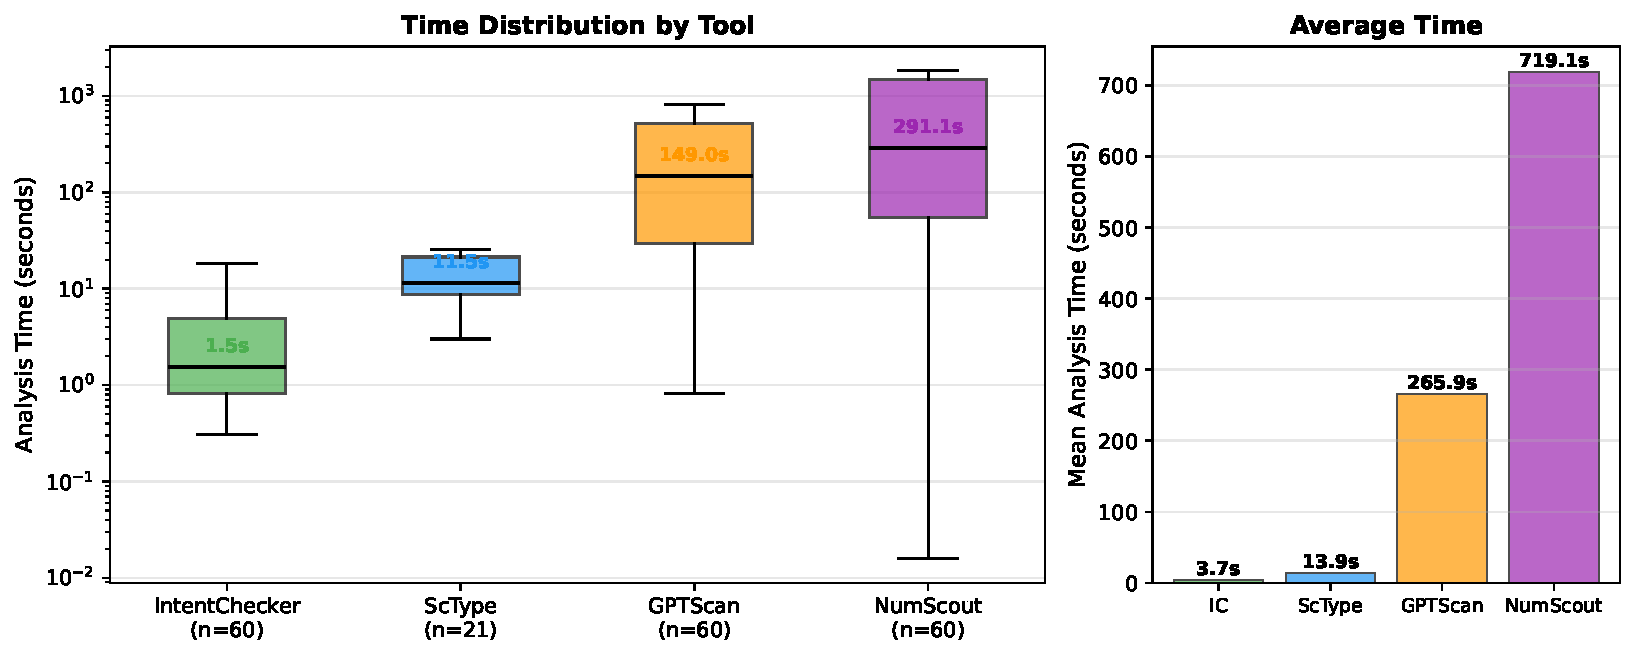
\includegraphics[width=\linewidth]{Fig9.pdf}
    \caption{Analysis time comparison across four tools (log scale). Left: box plot of per-case times over three runs. Right: mean analysis time.}
    \label{fig:rq3-time}
\end{figure}

\smallskip
\noindent\textbf{Position axis: when each tool is run.}
Fig.~\ref{fig:rq3-time} reports per-case analysis times pooled over three runs (60 observations per 20-case tool, 21 for ScType's seven applicable cases).
IntentChecker (mean 3.7\,s) and ScType (mean 13.9\,s) are both local, deterministic analyses that complete in seconds and produce identical times across the three runs.
By contrast, GPTScan (mean 266\,s) runs approximately 72$\times$ slower because its pipeline is sequential OpenAI API round-trips through a two-step LLM filter, and NumScout (mean 719\,s, median 291\,s) is slower still, with several cases running to NumScout's 1800\,s symbolic-execution timeout.
The box-plot spread visible in Fig.~\ref{fig:rq3-time} therefore comes entirely from these two LLM-driven pipelines, whose run-to-run variability is absent in the deterministic analyses.

\smallskip
\noindent\textbf{Synthesis.}
The two axes are not independent evaluation dimensions but the empirical shadow of the two structural constraints identified in \S\ref{sec:background}.
The criteria axis shows that the 20 mitigated cases sit outside the pattern and type catalogs of three tools, and that the reason is structural: criteria authored by tool designers admit only the shapes those designers anticipated, and numeric logic errors extend beyond any fixed anticipation.
The position axis shows that the latency envelopes of those tools are shaped by the post-hoc workflow they serve---audit and CI tolerate per-case latency in the minute range---while stepping into the development-time slot where the developer can still supply intent requires compressing that envelope by roughly two orders of magnitude. IntentChecker's observed 3.7\,s mean accordingly reads as a design-space requirement met rather than a speed advantage.
Taken together, IntentChecker occupies the joint corner of developer-authored criteria and development-time execution, the corner the two reversals jointly define.
Rather than competing with existing auditing-time detectors, it completes the detection design space by filling this development-time gap, which RQ1--RQ3 together characterize as both real and previously unoccupied.

\subsection{Threats to Validity}\label{sec:threats}

\noindent\textbf{Internal validity.}
The intent and debug annotations in RQ1 were authored by the researchers from the audit reports, not by the original developers. A different annotator could write a slightly different annotation, and an imprecise one could miss a bug a more precise annotation would catch.
This is mitigated by deriving each annotation directly from the audit report's stated root cause and recording it alongside each case in the supplementary material for independent re-evaluation.

\smallskip
\noindent\textbf{External validity.}
Our 89-case benchmark is drawn from Web3Bugs (Code4rena), NumScout (BNB Smart Chain), and Fly-in-the-Ointment. Together these sources cover a substantial portion of publicly documented Solidity numeric logic errors but are not exhaustive, and findings may not generalize to patterns absent from these curated sources.
The RQ1 correlation analysis is based on a small sample of $n=20$ mitigated cases, so the reported Pearson coefficients should be read as indicative trends rather than causal claims.

\smallskip
\noindent\textbf{Construct validity.}
RQ1's ``mitigation'' relies on the validation engine producing a Violated judgment on the buggy code rather than a downstream measurement of developer behavior. Whether a developer reading it would correctly diagnose and fix the bug is future work.
In RQ3, GPTScan mitigation results are taken from the per-contest breakdown published with Sun~et~al.~\citep{gptscan,gptscan_web3bugs} because GPTScan invokes OpenAI model aliases whose underlying snapshots have been redirected since 2023, and our April~2026 reruns produced rule activations at different functions than the published results. Per-case latency in Fig.~\ref{fig:rq3-time} uses our reruns for all four tools to ensure the same hardware, OS, and network conditions---the fair basis for latency comparison.
Running NumScout required a one-line source-code fix to its safeTransfer handler in \texttt{feature\_detector/semantic\_analysis.py}~\citep{numscout_semantic}, which otherwise crashed with an UnboundLocalError on some benchmark contracts. The fix renames a mis-referenced local variable and is external to NumScout's detection logic, so it does not affect its findings on the bugs under study.

\section{Discussion}\label{sec:discussion}

\subsection{Intent Annotation Guidelines}\label{sec:disc:guidelines}

Within the value-level intent model, the annotation grammar (§\ref{sec:design}) defines what can be written. The question that remains is when a developer should write which annotation.
The 20 mitigated cases and 14 L5 expressible cases reveal a recurring pattern: the most impactful annotations express what the code does not already make explicit---an omitted state update, an unchecked relation between output and input, or the mathematical intent behind a lossy arithmetic path.
Three non-obvious guidelines are distilled from this observation.

\smallskip
\noindent\textbf{Guideline 1: Enumerate state variables a function should affect, not just those it actually affects.}
Developers naturally reason about the code they wrote---the variables they explicitly assigned, the calls they explicitly made.
Bugs of omission arise precisely from this cognitive bias: a state variable that should have been updated was simply never mentioned.
After writing a function, the developer should list the state variables whose value the function is expected to change and add at least a directional annotation (@Post var(Entry\,$<$\,Exit) or @Post changed(var, true)) for each.
Crucially, this practice depends only on the developer enumerating expected effects, not on any prior knowledge of the specific bug.

\smallskip
\noindent\textbf{Guideline 2: Anchor output expectations to known quantities.}
Many functions with numeric outputs have a known relationship---a bound, an equality, or a monotonic relation---with quantities already in scope: input parameters, related state variables, or values derivable from specific input instantiations.
Encoding this relationship as a @During or @Post annotation catches wrong-implementation bugs where the code runs without error but produces a directionally wrong or out-of-bound result.
Examples include @Post \texttt{\_balances[to] <= amount} bounding the output against the transferred amount (RebaseProxy.mint), @During \texttt{\_principalWithdrawable <= \_totalLiquidityWithdrawable} comparing two related state variables (LenderPool.\_calcPrincipalWithdrawable), and @Post \texttt{returnExpression == \_balance - mapToken\_tokenAmount[\_token]} asserting the return against a state-derived formula (Pools.getAddedAmount).
Such an annotation surfaces bugs through a violated relation even when the developer cannot pre-specify the exact output value.

\smallskip
\noindent\textbf{Guideline 3: For multi-step arithmetic, annotate the result against the mathematically ideal expression, not the code as written.}
Solidity's integer division truncates at every intermediate step, and the resulting precision loss depends on the order of operations.
Code that reads amount.div(12).mul(5) may look correct, but the developer's actual intent is the mathematical value $\lfloor\text{amount} \times 5 / 12\rfloor$.
Writing the intent annotation with the multiplication-before-division ordering---@During result $\geq$ amount * 5 / 12---causes IntentChecker to compare the code's early-truncation path against a form that defers truncation to the final division, surfacing the precision gap automatically.

\subsection{Annotation Authoring Burden and Future Automation}\label{sec:disc:burden}

IntentChecker's mitigation results are conditional on the developer supplying intent and debug annotations.
This is by design: the entire approach is predicated on the developer making their intent explicit. Accordingly, IntentChecker requires direct authoring effort from the developer.

\smallskip
\noindent\textbf{Effort 1: writing intent annotations.}
The intent model requires the developer to articulate, in the grammar of @During/@Post annotations, what the function is supposed to do. This translation from a mental model of intent into grammar-expressible assertions is itself effort: the developer must decide which properties to assert at which program points and must express each assertion within the grammar's syntactic form.

\smallskip
\noindent\textbf{Effort 2: supplying debug annotations for realistic execution paths.}
Even for code whose intent is clear, IntentChecker can only analyze the path that the developer's debug annotations actually exercise.
Debug annotations require the developer to choose representative ranges for each entry-point value the function reads. Choosing ranges that miss the buggy region produces a false negative, while choosing ranges that are too wide invites widening and produces uninformative Warning judgments. Either way, Satisfied judgments hold only within the declared ranges.
This is the standard cost of any debugging paradigm---traditional debuggers also only execute the inputs the developer provides---and developers mitigate it by iteratively refining ranges when Warning results draw attention to specific sub-intervals.

\smallskip
\noindent\textbf{Future direction: LLM-assisted annotation suggestion and auto-repair.}
A natural way to lower both annotation-authoring efforts is to combine IntentChecker with a large language model that observes the same source the developer is editing.
For intent annotations, the LLM could generate candidate @During/@Post annotations from the partial code the developer is currently writing, conditioned on two paper-internal artifacts---the intent annotation guidelines (§\ref{sec:disc:guidelines}) as structural priors and the per-case annotated benchmark as in-grammar exemplars---and present them as suggestions the developer accepts or edits.
For debug annotations, the LLM could propose representative ranges from invocation patterns visible in the project under edit and from per-pattern range exemplars in the annotated benchmark.
Such annotation suggestions can reduce the manual authoring effort for both the 20 mitigated cases and the 14 L5 cases identified in RQ2 (Fig.~\ref{fig:rq1-limitations}).
A second direction proposes in-editor code repair: when IntentChecker returns a Violated judgment, the LLM suggests edits that bring the program's actual behavior within the developer's declared intent, for them to evaluate before committing.
Both directions are left as future work, building on this paper's intent model, validation engine, guidelines (§\ref{sec:disc:guidelines}), and per-case annotated benchmark.

\subsection{Current Limitations}\label{sec:disc:tech}

Beyond the annotation authoring burden discussed in §\ref{sec:disc:burden}, two tool-side technical boundaries and one methodological limit of the present evaluation remain.

\smallskip
\noindent\textbf{Contract-level intent.}
IntentChecker's intent model operates on individual functions within a single transaction.
A class of numeric properties, however, constitutes contract-level intent---properties that relate quantities established by different transactions across the contract's lifetime rather than within a single function execution.
The canonical example is the ERC20 conservation property totalSupply == sum(balances): any single function execution may temporarily increment one side and not the other, but across the entire transaction history the two must agree.
Another example is the price oracle manipulation pattern, where the buggy behavior only manifests when one transaction sets up state that a later transaction reads.
Capturing contract-level intent would require tracking state across transactions and aggregating across all balance entries, both of which lie outside the current function-level, single-transaction interval-domain analysis.

\smallskip
\noindent\textbf{Unsupported Solidity constructs.}
IntentChecker's Yul support targets arithmetic computation---add, sub, mul, div/sdiv, mod/smod, exp, comparison and bitwise operators, shifts, and the modular forms mulmod/addmod---which covers the cases where inline assembly is used as a faster substitute for high-precision integer arithmetic, by far the most common use case in DeFi libraries.
However, hand-written Yul that uses memory and storage opcodes (mload/mstore, sload/sstore), control flow (if, for, switch), or function definitions falls outside the supported subset and is conservatively treated as $\top$.
The same conservative treatment applies to a small number of Solidity constructs that the abstract interpreter does not model: abi.decode from raw bytes, keccak256, and other built-ins whose results depend on opaque cryptographic operations.
Bugs whose buggy/correct distinction depends on the precise value produced by such constructs are correspondingly out of IntentChecker's reach (these account for the L3 cases in Fig.~\ref{fig:rq1-limitations}).

\smallskip
\noindent\textbf{Evaluation methodology: developer study.}
This paper evaluates IntentChecker through structural analysis---what the tool can and cannot detect (RQ1), what the intent model can and cannot express (RQ2), and how the tool compares with existing detectors (RQ3)---rather than through a developer study measuring perceived usability or annotation intuitiveness.
A controlled study with Solidity-experienced participants would answer a complementary set of questions: whether developers find the annotation syntax natural, how long annotation authoring takes in practice, and whether the tool's feedback leads to faster bug discovery than existing debugging workflows.
Meaningful results for such a study require realistic development-time conditions~\citep{defisecurity}, which in IntentChecker's current form are dominated by two confounds: the manual annotation-authoring burden described in §\ref{sec:disc:burden}, which is specifically what the envisioned LLM-assisted suggestion layer is designed to reduce, and the analyzer coverage gaps above, which bias task selection toward cases the tool already handles.
The usability study is therefore deferred to after both the LLM-assisted annotation layer and the analyzer extensions are in place, where the study can assess the intended workflow rather than its current manual-authoring approximation.

\section{Related Works}\label{sec:related}
\subsection{Numeric Logic Error Detection in Solidity}
Logic error detection focuses on identifying discrepancies between developer intentions and actual program behavior in smart contracts.

\citep{highguard} addresses business logic violations in smart contracts by using Dynamic Condition Response (DCR) graphs
to model expected behaviors including temporal constraints, role-based access control, and inter-function dependencies.
The system monitors runtime transactions against user-provided DCR models and their function mappings,
generating violation reports when execution activities deviate from the specified business logic patterns.

\citep{smartpulse} verifies temporal properties of smart contracts by accepting user-specified Linear Temporal Logic (LTL) formulas
and attack models to check both safety and liveness properties.
The system not only detects violations but also generates concrete attack scenarios that demonstrate how the temporal properties can be violated,
providing developers with actionable insights into potential logic errors.

\citep{consolidating} enables developers to specify function and address behaviors using the ConSol syntax alongside their Solidity code,
then verifies whether the implementation adheres to these behavioral specifications and generates behavior-compliant Solidity programs without annotations.

\citep{smartinv} leverages multimodal learning to automatically infer invariants and detect machine unauditable bugs (MUBs)~\citep{exploitablebugs}
by analyzing both source code and natural language artifacts including comments, function signatures, and documented transaction scenarios.
The system employs a fine-tuned model with Tier of Thought (ToT) prompting that progressively predicts transaction contexts,
generates and ranks invariants, and ultimately identifies vulnerabilities through three-tier reasoning.

Furthermore, there are also approaches that address multiple transaction logic errors such as price manipulation~\citep{defiranger,defiguard,pomabuster,secplf,defitainter}
and flash loan attacks~\citep{defitail,midnight}.

The numeric logic error detectors above and IntentChecker differ along both axes identified in §\ref{sec:background}.2: who authors the detection criteria and when the tool is run.
Detectors that rely on pattern catalogs, language-model inference, or type rules are all designed to run over completed code, with criteria fixed at design time and applied post-hoc.
IntentChecker is positioned earlier in time and lets the developer declare intent explicitly through annotations evaluated inside the editor, crossing both axes simultaneously.
Because the two approaches see different inputs (code only vs.\ code with declared intent) and run in different workflow stages (post-hoc audit vs.\ development-time validation), their coverage is necessarily complementary.

\subsection{Specification-based Smart Contract Verification}
Specification-based verification approaches focus on verifying general properties and correctness requirements of smart contracts rather than specific developer intentions.

\citep{scribble} provides a framework that transforms developer annotations into Solidity assertion code,
enabling testing with existing tools like MythX~\citep{mythx} and Mythril~\citep{mythril}.
The framework supports multiple annotation types including if\_succeed (conditions for successful function returns),
invariant (contract-level properties that must always hold), if\_updated (conditions checked when state variables change),
and assert (validations at specific execution points), making formal specifications accessible through familiar testing pipelines.

\citep{smartace} builds upon Scribble~\citep{scribble} to verify whether Solidity code satisfies specifications written in the Scribble language,
leveraging C-based verification tools like SeaHorn~\citep{seahorn}, libFuzzer~\citep{libfuzzer}, and KLEE~\citep{klee} by transforming smart contracts into LLVM-IR based harnesses.
The framework abstracts the $2^{160}$ possible user addresses into a small set of representative users (implicit, transient, and explicit),
enabling verification of properties that must hold for arbitrary numbers of users, such as accounting properties like
"the contract balance equals the sum of all user deposits."

\citep{idealist} verifies Solidity code using two types of annotations: specification annotations (loop invariants, call invariants, and call modifies) that developers declare as assumptions,
and verification annotations (ensures, reverts\_if, and contract invariants) that the tool checks against the implementation.
The system assumes the truth of specification annotations and uses them to verify whether the code satisfies function post-conditions,
correctly handles revert conditions, and maintains contract invariants throughout execution.

\citep{solvent} focuses on verifying liquidity properties of smart contracts through formal methods
by converting both the contract code and user-defined liquidity properties into SMT constraints.
The system then checks whether the contract satisfies these properties using SMT solvers,
generating counterexamples when violations are detected to help developers understand potential liquidity issues.

While the specification-based approaches above provide dedicated specification languages and discharge verification obligations through SMT solving, symbolic execution, or assertion injection over completed code, IntentChecker's intent model occupies a different point in the design space.
First, its annotation language targets value-level numeric intent expressed as interval-valued relationships over specific variables and program points, whereas specification-based languages above express properties as Boolean assertions over types or contract state.
Second, its tri-valued validation engine (§\ref{sec:intent-semantics}) operates over the intervals produced by interval-domain abstract interpretation, which is light enough to run at development time as the developer writes code, whereas SMT-based and symbolic-execution-based checks are discharged as verification tasks after coding is complete.
Third, each annotation yields a graded outcome (Satisfied, Warning, or Violated) along with a risk score and the sub-intervals where the violation may occur, pointing the developer to the problematic value region rather than returning a binary verification verdict.
The two approaches are therefore complementary in specification style, verification backend, and workflow stage.

\subsection{Tools for Strengthening Security During Development Phase}
Development-phase security tools integrate vulnerability detection directly into the coding workflow, enabling developers to identify and address security issues as they write code rather than in post-development analysis.
\citep{making} presents an integrated development environment for smart contract development that combines natural language model-based code autocompletion with security validation.
The platform integrates existing static analysis tools including Oyente~\citep{oyente}, Mythril~\citep{mythril}, and Securify~\citep{securify} to provide comprehensive security reports during development workflow.

\citep{solhint} provides a Solidity linter that detects predefined vulnerability patterns including low-level calls, reentrancy, and deprecated function usage during development.
The tool enforces security best practices by checking for patterns such as proper visibility declarations, send result validation, and secure compiler version usage.

While these development-phase tools rely on design-time detection criteria for known vulnerability patterns,
IntentChecker enables developers to specify their intended numeric behaviors through annotations and validates whether the actual program execution matches the declared intent.

\section{Conclusion}\label{sec:conclusion}

This paper presents IntentChecker, a development-time value-level intent validation tool for Solidity built on SolQDebug and extended to a multi-contract single-transaction scope. The tool classifies developer-supplied @During/@Post intent annotations as Satisfied, Warning, or Violated against the abstract states produced by interval-domain analysis, grounded in a formal denotational semantics, and reports a risk score and the violated region per annotation.

On 75 effective benchmark instances drawn from Web3Bugs, NumScout, and the Greedy Contract dataset of \citet{flyinointment}, IntentChecker mitigated 20 cases by returning Violated judgments at a mean 3.69\,s per case (RQ1). RQ2 traced the remaining 55 cases to two levels of limitation. Of these, 21 are analysis-engine limits where the interval-domain state at the check point is too coarse to distinguish the bug. The other 34 are annotation-grammar limits rooted in two structural properties of the value-level intent model: value-level annotations can express a bug only when the corrective variable is in the function's scope, and algorithm-level bugs lie outside what a value-level grammar is designed to express. RQ3 then compared IntentChecker with existing detectors and empirically confirmed that their coverage and latency envelopes are bounded by both structural axes this paper identifies, namely who authors the detection criteria and when the tool is run.

These results position IntentChecker as complementary to existing detection tools: rather than competing on detection accuracy, it fills the development-time slot that auditing-time tools structurally cannot occupy. Future work targets LLM-assisted annotation suggestion and auto-repair, along with capturing contract-level intent.

\section*{Acknowledgements}
This work was supported by the Institute of Information \& communications Technology Planning \& Evaluation (IITP) grant funded by the Korean government (MSIT) (RS-2021-II210177, High Assurance of Smart Contract for Secure Software Development Life Cycle), the Technology development Program (RS-2025-25455127) funded by the Ministry of SMEs and Startups (MSS, Korea), and the ``Regional Innovation System \& Education (RISE)'' through the Seoul RISE Center, funded by the Ministry of Education (MOE) and the Seoul Metropolitan Government (2025-RISE-01-003-01).

\section*{Author Contributions}
Inseong Jeon participated in conceptualization, methodology design, system implementation, data collection, experiments, and manuscript writing. Sundeuk Kim and Hyunwoo Kim assisted in experiments, data collection and analysis, and contributed to manuscript writing. Hoh Peter In provided resources, assisted in editing the manuscript, and supervised the entire project. All authors reviewed and approved the final version of the manuscript.

\section*{Data Availability}
The benchmark of 89 real-world numeric logic error instances curated from Web3Bugs~\citep{exploitablebugs}, NumScout~\citep{numscout}, and the Greedy Contract dataset of \citet{flyinointment}, along with the IntentChecker implementation~\citep{intentchecker}, evaluation scripts, and experimental results, are available at \url{https://github.com/iwwyou/IntentChecker.git}.

\section*{Declarations}

\noindent\textbf{Competing interests} The authors declare no competing interests.

\noindent\textbf{Ethical approval} Not applicable since there are no human and/or animal studies included in this paper.


\begin{thebibliography}{99}

\bibitem[Arora et~al.(2024)]{secplf}
Arora, S., et al.: SecPLF: Secure protocols for loanable funds against oracle manipulation attacks. In: Proceedings of the 19th ACM Asia Conference on Computer and Communications Security (ASIACCS), pp. 1394--1405 (2024). https://doi.org/10.1145/3634737.3637681

\bibitem[Anthropic(2026)]{claude}
Anthropic: Claude. \url{https://www.anthropic.com/} (2026). Accessed April 2026

\bibitem[Bartoletti et~al.(2024)]{solvent}
Bartoletti, M., et al.: Solvent: liquidity verification of smart contracts. In: International Conference on Integrated Formal Methods (iFM), pp. 256--266 (2024). \url{https://doi.org/10.1007/978-3-031-76554-4_14}

\bibitem[Cadar et~al.(2008)]{klee}
Cadar, C., et al.: KLEE: unassisted and automatic generation of high-coverage tests for complex systems programs. In: OSDI, pp. 209--224 (2008). https://doi.org/10.5555/1855741.1855756

\bibitem[Chaliasos et~al.(2024)]{defisecurity}
Chaliasos, S., et al.: Smart contract and defi security tools: Do they meet the needs of practitioners?. In: Proceedings of the 46th IEEE/ACM International Conference on Software Engineering (ICSE), pp. 1--13 (2024). https://doi.org/10.1145/3597503.3623302

\bibitem[Chen et~al.(2025)]{numscout}
Chen, J., et al.: NumScout: Unveiling Numerical Defects in Smart Contracts using LLM-Pruning Symbolic Execution. IEEE Transactions on Software Engineering (2025). https://doi.org/10.1109/TSE.2025.3555622

\bibitem[NumScout(2026a)]{numscout_dataset}
NumScout: 95 Samples Experiment Dataset. \url{https://github.com/NumScout/NumScout/tree/main/Experiment/95_Samples_Run} (2026). Accessed April 2026

\bibitem[NumScout(2026b)]{numscout_semantic}
NumScout: feature detector source code (\texttt{semantic\_analysis.py}). \url{https://github.com/NumScout/NumScout/blob/main/feature_detector/semantic_analysis.py} (2026). Accessed April 2026

\bibitem[Consensys Diligence(2026a)]{mythril}
Consensys Diligence: Mythril. \url{https://github.com/ConsenSysDiligence/mythril} (2026). Accessed April 2026

\bibitem[Consensys Diligence(2026b)]{mythx}
Consensys Diligence: MythX. \url{https://mythx.io/} (2026). Accessed April 2026

\bibitem[Consensys Diligence(2026c)]{scribble}
Consensys Diligence: Scribble. \url{https://diligence.security/scribble/} (2026). Accessed April 2026

\bibitem[Eshghie et~al.(2024)]{highguard}
Eshghie, M., et al.: Highguard: Cross-chain business logic monitoring of smart contracts. In: Proceedings of the 39th IEEE/ACM International Conference on Automated Software Engineering (ASE), pp. 2378--2381 (2024). https://doi.org/10.1145/3691620.3695356

\bibitem[Feist et~al.(2019)]{slither}
Feist, J., Grieco, G., Groce, A.: Slither: A static analysis framework for smart contracts. In: 2019 IEEE/ACM 2nd International Workshop on Emerging Trends in Software Engineering for Blockchain (WETSEB), pp. 8--15 (2019). https://doi.org/10.1109/WETSEB.2019.00008

\bibitem[Gurfinkel et~al.(2015)]{seahorn}
Gurfinkel, A., et al.: The SeaHorn verification framework. In: International Conference on Computer Aided Verification, pp. 343--361 (2015). \url{https://doi.org/10.1007/978-3-319-21690-4_20}

\bibitem[Google(2026)]{gemini}
Google: Gemini. \url{https://gemini.google.com/} (2026). Accessed April 2026

\bibitem[Jeon et~al.(2025)]{solqdebug}
Jeon, I., et al.: SolQDebug: Debug Solidity Quickly for Interactive Immediacy in Smart Contract Development (2025). https://doi.org/10.21203/rs.3.rs-8077153/v1

\bibitem[IntentChecker(2026a)]{intentchecker}
IntentChecker. \url{https://github.com/iwwyou/IntentChecker.git} (2026). Accessed April 2026

\bibitem[IntentChecker(2026b)]{dappscananalysis}
IntentChecker: DAppSCAN contract analysis dataset. \url{https://github.com/iwwyou/IntentChecker/blob/main/evaluation/DappSCAN_contract_analysis/contract_analysis_table.xlsx} (2026). Accessed April 2026

\bibitem[IntentChecker(2026c)]{rq2supp}
IntentChecker: RQ2 supplementary material---L4/L5 case classifications and annotations. \url{https://github.com/iwwyou/IntentChecker/tree/main/evaluation/RQ2} (2026). Accessed April 2026

\bibitem[IntentChecker(2026d)]{rq1supp}
IntentChecker: RQ1 supplementary material---per-case annotation plans and rationale. \url{https://github.com/iwwyou/IntentChecker/tree/main/evaluation/RQ1/annotation_plans.md} (2026). Accessed April 2026

\bibitem[Kong et~al.(2023)]{defitainter}
Kong, Q., et al.: Defitainter: Detecting price manipulation vulnerabilities in defi protocols. In: Proceedings of the 32nd ACM SIGSOFT International Symposium on Software Testing and Analysis (ISSTA), pp. 1144--1156 (2023). https://doi.org/10.1145/3597926.3598124

\bibitem[Li et~al.(2025)]{defitail}
Li, X., et al.: Penetrating the hostile: Detecting defi protocol exploits through cross-contract analysis. IEEE Transactions on Information Forensics and Security 20, 11759--11774 (2025). https://doi.org/10.1109/TIFS.2025.3626979

\bibitem[LLVM(2026)]{libfuzzer}
LLVM: libFuzzer. \url{https://llvm.org/docs/LibFuzzer.html} (2026). Accessed April 2026

\bibitem[Luu et~al.(2016)]{oyente}
Luu, L., et al.: Making smart contracts smarter. In: Proceedings of the 2016 ACM SIGSAC Conference on Computer and Communications Security (CCS), pp. 254--269 (2016). https://doi.org/10.1145/2976749.2978309

\bibitem[Nguyen et~al.(2023)]{idealist}
Nguyen, T.D., et al.: An idealist's approach for smart contract correctness. In: International Conference on Formal Engineering Methods, pp. 11--28 (2023). \url{https://doi.org/10.1007/978-981-99-7584-6_2}

\bibitem[OpenAI(2026)]{chatgpt}
OpenAI: ChatGPT. \url{https://chatgpt.com/} (2026). Accessed April 2026

\bibitem[Pearson(2026)]{pearson_r}
Pearson correlation coefficient. \url{https://en.wikipedia.org/wiki/Pearson_correlation_coefficient} (2026). Accessed April 2026

\bibitem[Protofire(2026)]{solhint}
Protofire: Solhint. \url{https://github.com/protofire/solhint} (2026). Accessed April 2026

\bibitem[Ramezany et~al.(2023)]{midnight}
Ramezany, S., Setthawong, R., Setthawong, P.: Midnight: An Efficient Event-driven EVM Transaction Security Monitoring Approach For Flash Loan Detection. In: Proceedings of the 2023 20th International Joint Conference on Computer Science and Software Engineering (JCSSE), pp. 237--241 (2023). https://doi.org/10.1109/JCSSE58229.2023.10201970

\bibitem[Ren et~al.(2021)]{making}
Ren, M., et al.: Making smart contract development more secure and easier. In: Proceedings of the 29th ACM Joint Meeting on European Software Engineering Conference and Symposium on the Foundations of Software Engineering (ESEC/FSE), pp. 1360--1370 (2021). https://doi.org/10.1145/3468264.3473929

\bibitem[Soud et~al.(2024)]{flyinointment}
Soud, M., Liebel, G., Hamdaqa, M.: A fly in the ointment: an empirical study on the characteristics of Ethereum smart contract code weaknesses. Empirical Software Engineering 29(1), 13 (2024). https://doi.org/10.1007/s10664-023-10398-5

\bibitem[Stephens et~al.(2021)]{smartpulse}
Stephens, J., et al.: SmartPulse: automated checking of temporal properties in smart contracts. In: Proceedings of the 2021 IEEE Symposium on Security and Privacy (SP), pp. 555--571 (2021). https://doi.org/10.1109/SP40001.2021.00085

\bibitem[Sun et~al.(2024)]{gptscan}
Sun, Y., et al.: Gptscan: Detecting logic vulnerabilities in smart contracts by combining gpt with program analysis. In: Proceedings of the IEEE/ACM 46th International Conference on Software Engineering (ICSE), pp. 1--13 (2024). https://doi.org/10.1145/3597503.3639117

\bibitem[GPTScan(2023)]{gptscan_web3bugs}
GPTScan: Web3Bugs per-contest evaluation results. \url{https://github.com/MetaTrustLabs/GPTScan-Web3Bugs} (2023). Accessed April 2026

\bibitem[Tsankov et~al.(2018)]{securify}
Tsankov, P., et al.: Securify: Practical security analysis of smart contracts. In: Proceedings of the 2018 ACM SIGSAC Conference on Computer and Communications Security (CCS), pp. 67--82 (2018). https://doi.org/10.1145/3243734.3243780

\bibitem[Wang et~al.(2024a)]{defiguard}
Wang, D., et al.: Defiguard: A price manipulation detection service in defi using graph neural networks. IEEE Transactions on Services Computing (2024). https://doi.org/10.1109/TSC.2024.3489439

\bibitem[Wang et~al.(2024b)]{smartinv}
Wang, S.J., Pei, K., Yang, J.: Smartinv: Multimodal learning for smart contract invariant inference. In: Proceedings of the 2024 IEEE Symposium on Security and Privacy (SP), pp. 2217--2235 (2024). https://doi.org/10.1109/SP54263.2024.00126

\bibitem[Wei et~al.(2024)]{consolidating}
Wei, G., et al.: Consolidating Smart Contracts with Behavioral Contracts. Proceedings of the ACM on Programming Languages 8(PLDI), 965--989 (2024). https://doi.org/10.1145/3656416

\bibitem[Wesley et~al.(2022)]{smartace}
Wesley, S., et al.: Verifying Solidity smart contracts via communication abstraction in SmartACE. In: International Conference on Verification, Model Checking, and Abstract Interpretation, pp. 425--449 (2022). \url{https://doi.org/10.1007/978-3-030-94583-1_21}

\bibitem[Wu et~al.(2023)]{defiranger}
Wu, S., et al.: Defiranger: Detecting defi price manipulation attacks. IEEE Transactions on Dependable and Secure Computing 21(4), 4147--4161 (2023). https://doi.org/10.1109/TDSC.2023.3346888

\bibitem[Xi et~al.(2024)]{pomabuster}
Xi, R., Wang, Z., Pattabiraman, K.: POMABuster: Detecting Price Oracle Manipulation Attacks in Decentralized Finance. In: Proceedings of the 2024 IEEE Symposium on Security and Privacy (SP), pp. 3923--3942 (2024). https://doi.org/10.1109/SP54263.2024.00257

\bibitem[Zhang(2024)]{sctype}
Zhang, B.: Towards finding accounting errors in smart contracts. In: Proceedings of the IEEE/ACM 46th International Conference on Software Engineering (ICSE), pp. 1--13 (2024). https://doi.org/10.1145/3597503.3639128

\bibitem[Zhang et~al.(2024)]{nyx}
Zhang, W., et al.: Nyx: Detecting exploitable front-running vulnerabilities in smart contracts. In: Proceedings of the 2024 IEEE Symposium on Security and Privacy (SP), pp. 2198--2216 (2024). https://doi.org/10.1109/SP54263.2024.00146

\bibitem[Yang et~al.(2025)]{hyperion}
Yang, S., et al.: Hyperion: Unveiling DApp Inconsistencies Using LLM and Dataflow-Guided Symbolic Execution. In: Proceedings of the 2025 IEEE/ACM 47th International Conference on Software Engineering (ICSE), pp. 2125--2137 (2025). https://doi.org/10.1109/ICSE55347.2025.00015

\bibitem[Zhang et~al.(2023)]{exploitablebugs}
Zhang, Z., et al.: Demystifying exploitable bugs in smart contracts. In: Proceedings of the 2023 IEEE/ACM 45th International Conference on Software Engineering (ICSE), pp. 615--627 (2023). https://doi.org/10.1109/ICSE48619.2023.00061

\bibitem[Zheng et~al.(2024)]{dappscan}
Zheng, Z., et al.: Dappscan: building large-scale datasets for smart contract weaknesses in dApp projects. IEEE Transactions on Software Engineering 50(6), 1360--1373 (2024). https://doi.org/10.1109/TSE.2024.3383422

\bibitem[Zhou et~al.(2023)]{defiattacks}
Zhou, L., et al.: Sok: Decentralized finance (defi) attacks. In: Proceedings of the 2023 IEEE Symposium on Security and Privacy (SP), pp. 2444--2461 (2023). https://doi.org/10.1109/SP46215.2023.10179435

\end{thebibliography}


\end{document}
